% Master's Thesis
% by Rasmus Tibell

%\documentclass[a4paper]{article}
%\documentclass[draft]{article}
\documentclass[a4paper,11pt]{kth-mag}

\usepackage[T1]{fontenc}
\usepackage{textcomp}
\usepackage{lmodern}
\usepackage[latin1]{inputenc}
\usepackage[swedish,english]{babel}
\usepackage{nada-ex}

\usepackage{graphicx}
\usepackage{multirow}
\usepackage{mathtools}
\usepackage{multibbl}
\usepackage{float}
%\usepackage[titletoc]{appendix}
%\usepackage[table]{xcolor}
\usepackage{booktabs,caption,fixltx2e}
\usepackage[flushleft]{threeparttable}
\usepackage{wrapfig}
\usepackage{xspace}
% \usepackage[pdftex]{graphicx}


\title{Master's Project in Computer Science}
%\subtitle{Duis autem vel eum iruire dolor in hendrerit in}

\author{Rasmus Tibell}
\date{November 2014}
\blurb{Master's Thesis at NADA\\Supervisor: Tjoho\\Examiner: Tjohej}
\trita{TRITA xxx yyyy-nn}


\restylefloat{table}

\begin{document}

%===============
%= hypenations =
%===============
\hyphenation{social-demokratiska arbetare-parti}
\hyphenation{multi-layer persep-trons tourna-ment cross-over con-formal pre-diction gene-rations popu-lation}

\newbibliography{art}
\bibliographystyle{art}{unsrt} 

\newbibliography{dat}
\bibliographystyle{dat}{unsrt} 

\newbibliography{rdr}
\bibliographystyle{rdr}{alpha} 

%\maketitle
\frontmatter
\maketitle
%%
%% This is file `kth-abs.tex',
%% generated with the docstrip utility.
%%
%% The original source files were:
%%
%% kthesis.dtx  (with options: `abstract')
%% 
%% IMPORTANT NOTICE:
%% 
%% For the copyright see the source file.
%% 
%% Any modified versions of this file must be renamed
%% with new filenames distinct from kth-abs.tex.
%% 
%% For distribution of the original source see the terms
%% for copying and modification in the file kthesis.dtx.
%% 
%% This generated file may be distributed as long as the
%% original source files, as listed above, are part of the
%% same distribution. (The sources need not necessarily be
%% in the same archive or directory.)
\begin{abstract}
  This is a skeleton for KTH theses. More documentation
  regarding the KTH thesis class file can be found in
  the package documentation.
\end{abstract}
\endinput
%%
%% End of file `kth-abs.tex'.

\clearpage
\selectlanguage{swedish}
\begin{abstract}
  Denna fil ger ett avhandlingsskelett.
  Mer information om \LaTeX-mallen finns i
  dokumentationen till paketet.
\end{abstract}
\selectlanguage{english}
\clearpage
\tableofcontents
\mainmatter

%prekth%\pagebreak
%prekth%\tableofcontents


\pagebreak
\section{Introduction}

The research around neural networks in general and multilayer perceptrons in special has lead to many novel ideas that increases the quality of the predictions and reduced the running time of the alghoritm. That in combination with the gained knowledge in using multilayer perceptrons has opens new fields for there use. The question at hand is if a multilayer perceptron can predict the final selling price of a apartment in a co-operative housing societies sold in Stockholm city with reasonable accuracy. And can it outperform a more commonly used machine learning system like the support vector regression (SVR).
   

\subsection{Background}
The predicting power of the machine learning system has steadily increase over the years mainly due to intensive research that has refined and improved the underlying algorithms. The same development holds for the Multilayer Perceptrons but the path to the current abilities and performance has had it's ups and downs. In the early 1960's the perceptrons became popular and the expectations were high but 1969 Minsk and Papert analysed there limitations which dampened the enthusiasm. Adding hidden layers (multilayer) doesn't help to break theses limitations as long as they are linear. The power comes from the combination of multiple layers of hidden units using non-linear activation functions. One major restriction is that the perceptron learning algorithm is ill suited for neural networks with multiple layers of non-linear units. The solution came with the back-propagation algorithm that generalizes well with multilayer perceptrons with linear and non-linear units. Tough it is a bit misleading that they still are called multilayer perceptrons despite the fact that the perceptron algorithm is seldom used these days.
\\
Predicting the price of a house or a apartment is a classic and commonly used example within the machine learning community. This in combination with being a resident in Stockholm where as in many capital cities the state of the apartment market is on everyone lips. Even as a resident it is often hard to understand which factors are affecting the prices of apartments. The notion is that it probably is more complex to analyse the market of apartments in Stockholm then determine the housing price in other parts of Sweden. The idea was born to try to predict the prices of apartments for sale and to find some of the major factors affecting the final price. All data used in the project stems from public available sources, so called ``Open Data'' sources. This hopefully makes it easy for those who wants to lock into this machine learning example domain and experiment and draw there own conclusions from this work.
\\
There is a belief amongst some of the experts that the price for which the apartments are sold doesn't reflect the true value of the object. Prices has been constantly rising since the mid nineties and the proportion of the salary spent on living has increased for the habitants in the Stockholm area. The driving forces behind this is increasing GDP, low production of new apartments, the constant influx of people to Stockholm and a low rate of interest for apartment loans. All these factors together makes the market of apartment quite complicated and increases the complexity of predicting a accurate prices.


\subsubsection{Problem description}
This paper explores the feasibility of creating a machine learning model that can predict the price of a apartment sold in central Stockholm with a fare precision and based on a neural network of type Multilayer Perceptron with a hand full of contemporary techniques applied. The Multilayer Perceptron will henceforth often be shortened to MLP.
\\
\texttt{ToDo: Add more descriptive text...} 
\\

\subsubsection{Traditional pricing model} \label{sss:hedonic}
One of the most wide spread models used to analyse property values are the hedonic price model which often are used by condominium brokers, banks and lending institutions. This model is based on the assumption that apartments are not homogeneous but differs in there attributes and that this is reflected in the selling price where the buyer implicitly pays for these favourable attributes. The hedonic price equation can be written as:
\begin{equation} \label{eq:hedonic_pe_base} 
y_{i} = \beta_{j} X_{j,i}  + \epsilon_{i}
\end{equation}

In the above equation (\ref{eq:hedonic_pe_base}) $y_{i}$ is the $i$-th observed sales price where $i \in 1 \ldots N$, N is the number of sales. The implicit prices of the attributes mentioned above is found in $\beta$ where $j \in 1 \ldots F$, $X$ is the sales data and F is the number of attributes. Errors are capture by $\epsilon$ the error term. Attributes often encapsulates the characteristics of the apartment, location and features of the neighbourhood.  
\\
\texttt{ToDo: describe PCA process and results from Pearssons} 
\\


\subsubsection{Objective}
As mentioned before the goal as to find a machine learning model that can predict the selling price of an apartment situated in the centre of Stockholm. This has to be done with a good quality to be meaningful for the end user. This kind of model can be use by apartment agencies to predict the future selling price or by financial institutions (loan givers) to find out the value of the pledge. To construct the model a neural network of the type multilayer perceptron is used in combination with some novel techniques to increase the precision of the predictions. Below is a list of the techniques use:
\begin{itemize}
\item Gradient descent
\item MiniBatch
\item Early stopping
\item Adjustable learning rate and momentum
\item Random initialization of weights
\item Conformal Prediction
\end{itemize}
The performance of the produced model is compared with support vector regression (SVR) to verify that the multilayer perceptron can outperforms a regular SVR. 
\\
\texttt{ToDo: develop a MP-model} \\
\texttt{ToDo: describe selected parameters} \\

\subsubsection{Restrictions}
This paper will not describe the whole process of how to construct a full fledged application. Nor will it result in any deployable software solution.Though all the code snippets that are developed during this research will be made available as Open Source at github.com.
\\
\texttt{ToDo: Check that all restrictions is accounted for}\\





\pagebreak
\section{Literature Review} \label{ss:literature_review}
The literature review is divided into two parts, since the nature of the reviewed papers naturally falls into two categories; research in the apartment and housing market domain and theory and techniques applicable to machine learning. 
\\
In the first part of this chapter studies regarding pricing structure and factors affecting the final pricing are reviewed. This part of the review is structured on a per article basis, the main reason for selecting this strategy is the diversity of the perspectives in the reviewed papers. The goal is to identify the main factors affecting the pricing of apartments and explore the relevant knowledge in the field accumulated in previous research. 
\\
The second part considers articles discussing novel techniques to improve predictions and performance of neural networks, common practices used when evaluating models and recommendations concerning tuning and parameter adjustments. For these topics the reviews are performed on a per subject basis and each subject is covered in a separate section.
\\

\subsection{Review of literature covering apartment and housing markets} 
All papers reviewed in this section share the common opinion that real estate assets and apartments are heterogeneous to there nature. The price may be affected by hundreds of factors and that many different outcomes are possible due to buyers preferences, available information and circumstances of sale. This gives rise to the fact that the price of a property in a given point in time can be modelled as a random variable and a random error. 
\\
\texttt{ToDo: Add text discussing conclusions regarding the market} 

%=====
%= A prominent role in society 
%=====
\subsubsection{A prominent role in society}
As predictive models used to estimate values of apartments and real estates get more exact they are more likely to play a more prominent role in society and politics. In the article \cite{art}{WilsJoneJenkWare:04} the authors argues for the importance of a firm pricing model. The situation on the Swedish market has many similarities with the UK market discussed in the paper. Residential properties are mortgaged in about sixty-file percent in the UK market. Lenders use the current market price as the key metric for determining the lending ceiling which fuels the risk of overheating the market. This can inflict socio-economic damages and big losses for credit institutions. These problems have been observed in vulnerable countries in Europe.
A metric with a more sustainable value could reduce the risk of over heating and would be preferable. For this scenario to be plausible the predictive models has to be refined and give a prudent price estimate of the property. 



%=====
%= Crimes impact on apartment prices
%=====
\subsubsection{Crimes impact on apartment prices}
In the study of crimes impact on apartment prices in Stockholm \cite{art}{CeccWilh:11}, Caccato and Wilhelmsson concludes from there findings that the apartment price is expected to fall by 0.04 per cent for each per cent in increased crime rate. The decrees in prices rises to 0.21 per cent for each per cent increase in crime rate if only residential burglary is considered. Although the effect is not homogeneous over space, apartment prices are often affected to a lower degree in the central part of Stockholm compared to the outskirts. Taking this knowledge into concern in combination with the fact that this report is targeted against apartment in the central part of the city instigated the decision to exclude crime rate and resembling data from this work. Although several feature related approaches referred to by Caccato and Wilhelmsson are used in the model or has inspired feature selection in our work.  
\\
This study is based on 9,622 sale transactions of condominiums in Stockholm during 2008, data was supplied by M{\"a}klarstatistik AB. To enrich the dataset with supplementary features cross-sectional data from the Stockholm Police, Stockholm Statistics and the municipal of Stockholm was merged together with the sales transactions. The information was then used to form features like proximity to water, underground stations, crimes per 10.000 citizens and other characteristics of the neighbourhood. Geographical data was used to divide the region into four quadrants with the central business district (CBD) as a centre point, the distance between the given apartment and the centre point is also used as an feature. Due to the fact that effects of crime can spill-over to neighbouring areas Caccato and Wilhelmsson has incorporated so called lagged variables, these are weighted averages of values for neighbouring locations. This type of feature is not used in this paper, this follows from the fact that no crime statistics are use. Table \ref{tab:feature_list_CeccWilh_11} contains a condensed list of the attributes used.
\\
\begin{table}[H]
%\centering
\begin{tabular}{ | l || l | } 
\hline 
\multicolumn{2}{|c|}{Feature group} \\
\hline
\hline
Transaction price & Living area \\
Number of rooms & Monthly fee \\
Age of building (\#6) & Newly built \\
Elevator in house & Balcony belonging to apartment \\
Apartment at top floor & Apartment at first floor \\
\hline
Distance to CBD & North-east quadrant \\
North-west quadrant & South-west quadrant \\
\hline
Distance to water (\#3) & Distance to underground station (\#3) \\
Distance to highway (\#3) & Distance to main street (\#3) \\
\hline
Crime rate & Rate of robbery \\
Vandalism & Outdoor violence \\
Residential burglary & Shoplifting \\
Drug related crime & Theft \\
Theft of cars & Theft from cars \\
Assaults & \\
\hline
\end{tabular}
\caption{List of features used by Caccato and Wilhelmsson}
\label{tab:feature_list_CeccWilh_11}
\end{table}


%=====
%= Traditional real estate valuation
%=====   
\subsubsection{Traditional real estate valuation} \label{sss:traditional_valuation}
The real estate market and there valuation methods are described in the article \cite{art}{Kumm:13} by Max Kummerow at Curtin University. In this paper he elucidates the theory behind the methods used by the real estate market in USA. Valuation methods can be divided into two main categories: objective and subjective where the objective method stems from the rational paradigms of science in contrast to the subjective method that can be viewed as more of a ``art''. The fundamental properties of the objective method is that conclusions are based on evidence that when viewed by others the same result should be derived. Often the property price is perceived as a random variable this induce the notion that there are no ``true value'' of the properties price, rather there are multiple prices that are possible with varying probability.   
\\
The heterogeneity in the market gives rise to models based on price differences. These models uses selected sets of previous sales with similar characteristics, those that affects the price are identified and there value is estimated in order to calculate the price implication. This model is based on the notion that for complex product the customer pays for the utility and the price paid is the sum of the utility of the characteristics. Two types of errors arises in this model: random variation in sales price and estimation errors for the value implication, the total error is the sum of the two. Let $\sigma$ be the standard deviation of the price distribution and n the sample size of sales. Then the standard deviation of the mean is $\frac{\sigma}{\sqrt{n}}$ and decrees as the sample size increases. Due to the heterogeneity of the properties the variance $\sigma^{2}$ increases when the sample size increases. This leads to a error trade-off when increasing the sample size the variance $\sigma^{2}$ of the sample increases while the mean of the sampling distribution decreases.
\\
One commonly used model is the hedonic price model described in chapter \ref{sss:hedonic}, hedonic stems from Greek and means pleasure. The equation is written as: $y_{i} = \beta_{j} X_{j,i}  + \epsilon_{i}$ where 
$y_{i}$ is the i'th observed sales price $i \in 1 \ldots N$, N is the number of sales, $\beta$ is the implicit prices, $X$ contains the sales information, F is the number of attributes and $j \in 1 \ldots F$. Errors are capture by $\epsilon$ the error term. The fundamental principle in the hedonic price model is that buyer acquires a bundle of characteristics for whom she is willing to pay a certain amount for each of the them.
\\
In the article \cite{art}{Kumm:13} by Kummerow he refers to economic theory that states that the long running cost relates to the value and that the supply will be adjusted until price and cost is at equilibrium. Though the adjustment is protracted due to the time required for exploration and construction of housing which causes the market to seldom be at equilibrium hence the cost does not equal price for a lengthy period of time. The driving factor of the short term price is the supply and demand and the actual sales transaction is a necessity to disclose the price and cost relationship.  


%=====
%= Real estate valuation using neural networks
%=====
\subsubsection{Real estate valuation using neural networks} \label{sss:using_ann}
Artificial Neural Networks (ANN) are well suited to construct models used to predict real estate values. The networks ability to catch non-linear behaviours is on of its aptitudes to predict prices of apartments and houses. Many factors affecting the hosing market like inflation, social concerns and interest rates are non-linear. Another beneficial feature of the neural networks are there ability to cope with noisy data sets. In a study \cite{art}{MahaBakeNorw:99} performed on the Malaysian hosing market based on data from a time period of tree years (1994-1996) in total 300 sales (15\% used for validation and 5\% for testing), a MLP was used to predict the prices of terrace houses using nine features (sample year, land area, type of house, ownership type, build area, age of house, distance from city, environment and building quality). The network was configured with nine input nodes corresponding to the input features, a hidden layer comprising of 3 to 7 nodes and a single predicting output node. Using this method a root mean square error of 0,061717 was obtained for a MLP with five hidden units and a linear activation function. Both the hyperbolic tangent function and the sigmoid function produced results with higher error rate. The results obtained in the study indicates that the MLP is well suited for the task of predicting house prices and that it can outperform a multiple regression based algorithm.     
\\
\texttt{ToDo: More stuff from article about GA and Gamma Test ...}
\\
A more elaborate approach is discussed in the paper \cite{art}{WilsJoneJenkWare:04} where a Gamma Test (GT) is used to drive a Genetic Algorithm (GA) in the process of selecting useful features from a data set. This data was then used to train a ANN on the root mean squared error produced by the GT. Without any prior knowledge of the system the Gamma Test is able to estimate the noise level in the data, a quality measure that indicates whether a smooth model exists or not.This approach has the advantage of being able to handle dataset with large numbers of useful input but with high levels of noise or sparse data. Finding a good combination of features is a optimization problem and here a Genetic Algorithm is used to search for the optimal feature set. To find the optimum the GA uses a population of individuals who each has there own genome describing there characteristics. A objective function is used to estimate the individuals quality whit respect to the problem at hand. The algorithm evolves as the generations progresses. For every generation the population is adjusted where lower ranking individuals are excluded and new crated by a mating process where genome parts are exchanged (crossover)between spouses and with a small probability a mutation is performed. To be able to mate the individual has to succeed in a tournament. Here the genome is a boolean mask indicating whether the column of the data should be in the feature set or not. The objective function is quite complex in this paper but in essence it calculates the Gamme statistics for the genome, hence the included columns in combination with weighted measures of: the amount of noise, complexity of underlying relationships between output and input date and finally the complexity of the ANN layout.   

%=====
%= Condominium price estimation using open data
%=====
\subsubsection{Condominium price estimation using open data} \label{sss:using_open_data}
Price estimation using support vector regression (SVR) and Open Data from the New York condominium market is explored by \cite{art}{ArulMora:13} Arul and Morales in there paper. Initial they use a 10 dimensional data set with features related to the price containing 4950 data points from 2011 and 2012. There principal components analyse yielded 7 features that could account for 98,3\% of the data, high ranking features were: building classification, construction year, gross income and expense per square foot. The SVR based model based on the 10 open data features predicted prices with an average error of 38,2\%, further 36,11\% of the predictions where within 15\% of the actual price. In order to improve the predictions GPS based location data was included in to the data set as a distance to a origin point. This in combination with a feature selection gave a average error of 21,8\% where 49,1\% of the predictions fell into the 15\% range of the actual price. In the conclusion, it is suggested to include features regarding: crime data, school district data and socio-economic data.    

%===================
%===================
%=== Review of literature in the field perceptrons and machine learning
%===================
%===================
\subsection{Review of literature in the field perceptrons and machine learning}


%=====
%= Difficulties training neural networks
%=====
\subsubsection{Difficulties training neural networks} \label{sss:glorot_and_bengio}
One of the pit falls when training Neural Networks is to select a good regime for weight and bias initialization in combination with activation function. These issues are covered by X. Glorot and Y. Bengio in there paper \cite{art}{GlorBeng:10} where they study the effect of random initialization of weights and how the effects the gradient descent algorithm. The Sigmoid activation function has a non-zero mean and this is known to cause singular values in the Hessian matrix. They further discovered that the last hidden layer rapidly obtain there saturation value of 0 and that this situation can last very long. This makes the Sigmoid activation function less suitable for MLP:s and especially used in combination with the traditional initialization schema described by equation \ref{eq:weight_init_regular} in chapter \ref{sss:weight_bias_initialization}. The recommendation is to use the hyperbolic tangent or softsign activation function in combination with the so called normalized initialization, see equation \ref{eq:weight_init_normalized} in chapter \ref{sss:weight_bias_initialization}. Effects of changing the schema for weight initialization are explored in chapter \ref{sss:boosting_mlp_weight_init}. Further Glorot and Bengio concludes that the normalized initialization is well suited for the hyperbolic tangent activation function.    


%=====
%= Using dropout on hidden nodes
%=====
\subsubsection{Using dropout on hidden nodes} \label{sss:using_dropout}
In the paper \cite{art}{HintSrivKrizSutsSala:12} Improving neural networks by preventing co-adaptation of feature detectors G. Hinton et al. describes the regime of using ``dropout'' to avoid ``overfitting''. This is achieved by randomly omitting 50\% of the training data on the hidden nodes for each training case. When the model is used to predict e.g. verification or test data the outgoing weights has to be compensated by dividing them by 2, this because when predicting all the nodes are on unlike in the training phase. Additional improvement can be obtained by randomly dropping out 20\% of the inputs.  
This regime can also be viewed as a method of averaging different models. Significant improvement is shown for this method on e.g. the MNIST data set. 


%=====
%= Inductive Conformal Prediction
%=====
\subsubsection{Inductive Conformal Prediction} \label{sss:ref_conformal_prediction}
\cite{art}{Papa:08}
\cite{art}{PapaHara:10}
\cite{art}{PapaVovkGamm:07}
\cite{art}{PapaVovkGamm:11}
\cite{art}{ShafVovk:08}
\texttt{ToDo: More stuff...}


\texttt{References ToDo}
\cite{art}{CaplChopLeahLecuTham:08}
\cite{art}{ChopThamLeahCaplLeCu:07}





\pagebreak
\section{Method}
% ToDo: General text about the method...
In this chapter the the methodology that was used to facilitate the making of this master thesis is describe. 
Finding appropriate feature candidates was one of the first challenges faced in this work. There are a significant amount of papers discussing potential candidates to bring in to the model, those with similar conditions has inspired the selection of features and they are reviews in chapter \ref{ss:literature_review}. When the selection of features was completed a search for appropriate data sources begun. All the required information was found from open data source. To facilitate the data capture and transformation a toolbox of shell- and Python scripts was created. Generation of the feature space was performed by a Scala application that rendered the features to the database and for future processing by Weka. In this stage the features were normalised and abnormal records where dismissed. For a detailed description of this process see chapter \ref{sss:data_cleansing}. The built in PCA and MLP functionality of Weka was used to select the features that contributed most to the solution of the model. Weka was enriched with a hyperbolic tangent activation function to promote the ability to capture the non-linearities in the model, see chapter \ref{sss:weka_tanh} for further details. Early testing indicated that hyperbolic tangent outperformed the traditional sigmoid activation function, both with respect to the performance of the model and the speed of convergence of the gradient decent algorithm. Finally the selected features was exported to Weka's native file format ``arff''.
\\
Comparison with a more traditional machine learning algorithm is one of the major prerequisites of this paper. To stage this a commonly used Python library named LibSVM was used. A Python script reads the Weka data file (arff), partitions it into three parts, builds the model and validates it. Tuning of the SVR was done by iterating over a separate interval for each parameter searching for the appropriate values by evaluating the model against the test data set. As the icing on the cake some additional traits are added to the multilayer perceptron calculations like: conformal predictions, random initialization of weights, adjustable learning rates and momentum. Finally the parameters for the MLP algorithm is fine tuned and the definitive result is presented in chapter \ref{ss:results}.  
\\

The main features of the work flow is as follows: 
\begin{itemize}
\item Identify potentially useful features to include in model
\item Find data sources for features
\item Capture data from selected sources
\item Generate feature space
\item Perform principal components analyse (PCA) on features 
\item Select features for model
\item Compare performance between multilayer perceptron (MLP) and support vector regression (SVR)
\item Incorporate additional functionality to multilayer perceptron
\item Fine tune multilayer perceptron parameters
\item Evaluate result
\end{itemize}

%========================================
%===
%=== Data collection
%===
%========================================
\subsection{Data collection}
All data sources used in this research are publicly available, so called ``Open Data''. The Swedish parliament has issued a directive that requires all government departments and municipality's to make there data publicly available. This is one of the major reasons behind the rich variety of information available from the municipality of Stockholm witch is one of the major information sources.  
\\
The information gathering is done incremental starting with the retrieval of a list containing the streets of central Stockholm from the website svenskagator.se \cite{dat}{Sven:13}. This list is read into the MySQL database handling the persistent data, see chapter \ref{sss:street_load}. The list of streets are then used to fetch the final prices of sold apartments for the given time period, one a per street basis from slutpris.se \cite{dat}{Slut:13}. For details see chapter \ref{sss:slutpris}.

%***
%* Streets searched for sales
%***
\subsubsection{Streets searched for sales} \label{sss:street_load}
Street names from svenskagator.se \cite{dat}{Sven:13} is read from the site using the unix command line tool curl and processed by a born shell script that produces a SQL file witch contains insertion statements. This file is then used to load the MySQL database with the street names. In total 1341 street names is read into the database.
\\

%***
%* Apartment sale statistic
%***
\subsubsection{Apartment sale statistic} \label{sss:slutpris} %from slutpris.se
Information from the REST API at slutpris.se \cite{dat}{Slut:13} is structured according to the Json standard. A program written in Scala is used to retrieve the information from slutpris.se. For each street in the list specified in chapter \ref{sss:street_load} a separate HTTP request has to be performed, the response is retrieved, parsed and transformed into class instances that are stored in the database. The request URL and parameters for the REST call is as specified in table \ref{tab:slutpris_se}. Features collected from slutpris.se is described in table \ref{tab:slutpris_se_result}. 

\begin{table}[H]
\centering
\begin{tabular}{ |p{2cm}|p{2cm}|p{2cm}|p{2cm}| } 
\hline
\multicolumn{4}{|c|}{http://slutpris.se/main\_application/get\_search\_result/} \\
\hline
dateLimit & order & minrum & maxrum \\
minarea & maxarea & minpris & maxpris \\
minavg & maxavg & area &  \\
\hline
\end{tabular}
\caption{Request to slutpris.se}
\label{tab:slutpris_se}
\end{table}


\begin{table}[H]
%\centering
\begin{tabular}{ | p{5.6cm} | p{5.6cm} | } 
\hline 
\multicolumn{2}{|c|}{Feature} \\
\hline
Construction year of building & Building has elevator \\
Fireplace in apartment & Apartment has a duplex \\
Apartment is a penthouse & Apartment has balcony \\
Date of transaction & Price per square meter \\
Area in square meters & Number of rooms, kitchen excluded \\
Stores from the street level & Monthly fee payed to association \\
Selling price & Latitude and longitude coordinates \\
Street address of apartment & Name of reltor \\
Reltor identification &  \\
\hline
\end{tabular}
\caption{Attributes in response from slutpris.se}
\label{tab:slutpris_se_result}
\end{table}

Apartment statistics are gathered for transactions finalized in the time frame 2011-08-01 until 2013-06-08. In total about 8900 transactions are fetched from slutpris.se, they are then filtered and only apartments in the bounding box defined in table \ref{tab:sthlm_bounding_geobox}. For more information regarding the generation and cleaning of the data se chapter \ref{sss:data_cleansing} and \ref{sss:feature_aggregation} respectively.

\begin{table}[H]
%\centering
\begin{tabular}{ | l | l | l | } 
\hline 
Type & Min & Max \\
\hline
Latitude & 59.298149 & 59.356296 \\
Longitude & 18.021784 & 18.115082 \\
\hline
\end{tabular}
\caption{Bounding box of centre of Stockholm}
\label{tab:sthlm_bounding_geobox}
\end{table}


%***
%* Street information
%***
\subsubsection{Street information} \label{sss:street_info}
Information retrieved from slutpris.se is enhanced with the zip code and latitude and longitude are replaced with more accurate information retrieved from the open data portal of Stockholm's municipal, openstreetws.stockholm.se \cite{dat}{smos:13}. Sales statistics are sparse compared to the number of unique street addresses in the surveyed area. Those a lazy evaluating solution is more efficient then pre loading all the adequate data prior to the substitution. The solution is based on a caching schema that uses the database to persist the retrieved information. When a street address is searched a lookup in the cache is done, if the information is available in the cache it is returned to the requester. If the street address is not in the cache it is retrieved from Stockholm's open data portal.  Enhancement of the sales statistic is achieved by looping throw all entry's of the sales statistic and for each entry lookup the street information from the cache. 

%***
%* Historic inflation figures
%***
\subsubsection{Historic inflation figures} \label{sss:hist_inflation}
Statistics over the apartments sales is derived from a two year period and therefore inflation has an impact on the sales price over time, closed sales from 2011 would appear to have a actual lower price then more resent deals. To avoid this bias on the price feature the final sales price is adjusted according to the monthly inflation up to the last date of the examined time interval. Inflation statistics was retrieved from the Statistics Sweden (SCB) who is responsible for the official inflation figures. Information regarding the inflation rate \cite{dat}{Scb2:13} and underlying inflation rate \cite{dat}{Scb1:13}. The retrieved information is pre processed by a Python script and then read into the database.  

%***
%* Interest rates for apartment loans
%***
\subsubsection{Interest rates for apartment loans} \label{sss:interest_rates}
There is a ongoing debate regarding the interest rates influence on the sales price of apartments in Stockholm. The prerequisite for being able to examine whether the interest rate has an impact on the sales price, historical interest rates were fetched from Skandinaviska Enskilda Banken (SEB) \cite{dat}{SEB:13} and Swebank \cite{dat}{Sweb:13}. This information was temporary stored as CSV-files, pre processed by a Python script and inserted into the database. 

%***
%* National election result
%***
\subsubsection{National election result} \label{sss:election_stats}
Political preferences of buyers, neighbours and policies of governing parties is a potential feature that affects the market. Statistics from the previous Swedish election in 2010 and geographic information of the layout of the constituency's are available from the Swedish authority Valmyndigheten \cite{dat}{Valm:13}. This statistics were downloaded as Excel files and loaded into the database via a Python script. Geographic information regarding the constituency's layout is supplied as so called shape files. The coordinates is transformed and the GeoTool Java library is used to find out witch constituency a given apartment belongs to and its unique id. Finally this id is used to find the election figures from the database.

%***
%* Local features
%***
\subsubsection{Local features} \label{sss:local_features}
Stockholm's municipal \cite{dat}{sthlm:13} provides data about over eighty local feature types. Fourteen of those were selected as candidates for the models feature space. Each feature has a unique identifier that has to be fetched from a catalogue using REST-calls. This catalogue was retrieved whit the unix tool curl and stored in XML-format, a Python script reads the file en inserts the unit types into the database. A second Python script reads the entries of the selected feature types from the REST-service and stores them into the database. Each feature entry is associated with a geographic coordinate (latitude and longitude), this information is used when the feature space is generated to calculate the distance to the nearest feature of each type.   

\begin{table}[H]
%\centering
\begin{tabular}{ | l | l | } 
\hline 
\multicolumn{2}{|l|}{http\://api.stockholm.se} \\
\hline
\hline
Type & URL \\
\hline
unit types & /ServiceGuideService/ServiceUnitTypes \\
unit entry & /ServiceGuideService/ServiceUnitTypes/\{id\}/ServiceUnits \\
\hline
\end{tabular}
\caption{REST services at api.stochlolm.se}
\label{tab:feature_rest}
\end{table}


%========================================
%===
%=== Features
%===
%========================================
\subsection{Features} \label{sss:features}
The features can be classified into six major groups depending on there data domain and origin. The groups are in order taken from table 
\ref{tab:feature_list1}: sales information regarding the apartment, geographical reference information, distance to local feature units and from table
\ref{tab:feature_list2}: geographic position, interest rates, election result from 2010. A complete listing of all the features used to create the model can be found in appendix \ref{sss:appendix_a}.

%***
%* 
%***
\subsubsection{Feature aggregation} \label{sss:feature_aggregation}
At the point in time when the generation of the feature space occurs all the required data has been loaded into the database.
\\
\texttt{ToDo: More stuff...}

%\subsubsection{Description of Features} \label{sss:feature_description}
%\begin{table}[H]
%\centering
\begin{tabular}{ | l | l | p{7cm} | } 
\hline 
Nr & Feature & Description \\
\hline
\hline
1 & construction\_year & Year when the building was constructed \\
2 & elevator & Building has elevator installed \\
3 & fireplace & Fireplace available in apartment \\
4 & duplex & Apartment has a duplex \\
5 & penthouse & Apartment is a penthouse \\
6 & balcony & Apartment has balcony \\
7 & squares & Area of apartment in square meters \\
8 & rooms & Total number of rooms, kitchen excluded \\
9 & floor & Apartments floor, numbers of stores from the street level \\
10 & fee & Anual fee payed to the housing association \\
11 & agencyid & Reltor identification \\
\hline
12 & postal\_code & Zip code \\
13 & fix\_point\_1 & Distance in meters to KTH Royal Institute of Technology \\
14 & fix\_point\_2 & Distance in meters to The Royal Palace of Stockholm \\
15 & fix\_point\_3 & Distance in meters to Sergels Torg (CBD) \\
\hline
16 & jog\_track\_dist & Distance in meters to nearest jogging track \\
17 & pad\_pool\_dist & Distance in meters to nearest wading pool \\
18 & daycare\_dist & Distance in meters to nearest daycare center \\
19 & pool\_dist & Distance in meters to nearest pool facility \\
20 & open\_daycare\_dist & Distance in meters to nearest daycare center \\
21 & sports\_hall\_dist & Distance in meters to nearest sports hall \\
22 & outdoor\_gym\_dist & Distance in meters to nearest out door gymnasium \\
23 & sports\_field\_dist & Distance in meters to nearest sports field\\
24 & playing\_field\_dist & Distance in meters to nearest palying field \\
25 & library\_dist & Distance in meters to nearest common library\\
26 & env\_station\_dist & Distance in meters to nearest environment station \\
27 & preschool\_dist & Distance in meters to nearest preschool \\
28 & bath\_dist & Distance in meters to nearest bath facility \\
29 & playground\_dist & Distance in meters to nearest play ground \\
30 & subway\_dist & Distance in meters to nearest subway station \\
31 & station\_dist & Distance in meters to nearest train or commuter train station. \\
32 & park\_dist & Distance in meters to nearest park \\
33 & forest\_dist & Distance in meters to nearest forest \\
34 & water\_dist & Distance in meters to nearest watercourse \\
\hline
\end{tabular}
\caption{List of features part 1}
\label{tab:feature_list1}
\end{table}

\begin{table}[H]
%\centering
\begin{tabular}{ | l | l | p{7cm} | } 
\hline 
Nr & Feature & Description \\
\hline
\hline
35 & lat & Latitude given as decimal number coded in WGS84 \\
36 & lng & Longitude given as decimal number coded in WGS84 \\
37 & zone1 & Id of grid square where apartment is located, taken from a 7x7 grid. \\
38 & zone2 & Id of grid square where apartment is located, taken from a 9x9 grid. \\
\hline
39 & seb\_interest\_3m & SEB's interest rate for a 3 month bound loan when the apartment was sold \\
40 & seb\_interest\_2y & SEB's interest rate for a 2 year bound loan when the apartment was sold \\
41 & seb\_interest\_5y & SEB's interest rate for a 5 year bound loan when the apartment was sold \\
42 & seb\_interest\_10y & SEB's interest rate for a 10 year bound loan when the apartment was sold \\
43 & swebank\_interest\_3m & Swebank's  interest rate for a 3 month bound loan when the apartment was sold\\
44 & swebank\_interest\_2y & Swebank's interest rate for a 2 year bound loan when the apartment was sold \\
45 & swebank\_interest\_5y & Swebank's interest rate for a 5 year bound loan when the apartment was sold \\
46 & swebank\_interest\_10y & Swebank's interest rate for a 10 year bound loan when the apartment was sold \\
\hline
47 & proc\_M & Proportion of votes in local constituency won by Moderata samlings\-partiet \\
48 & proc\_C & Proportion of votes in local constituency won by Centerpartiet \\
49 & proc\_FP & Proportion of votes in local constituency won by Folkpartiet Liberalerna \\
50 & proc\_KD & Proportion of votes in local constituency won by Kristdemokraterna \\
51 & proc\_S & Proportion of votes in local constituency won by Sveriges social\-demo\-kratiska arbetare\-parti \\
52 & proc\_V & Proportion of votes in local constituency won by V{\"a}nsterpartiet \\
53 & proc\_MP & Proportion of votes in local constituency won by Milj{\H o}partiet de Gr{\H o}na \\
54 & proc\_SD & Proportion of votes in local constituency won by Sverige\-demokraterna \\
55 & proc\_Alians & Majority for the Alliance parties \\
56 & proc\_RodGron & Majority for the opposition parties \\
57 & majority\_Alians & Proportion of votes to the majority \\
\hline
\end{tabular}
\caption{List of features part 2}
\label{tab:feature_list2}
\end{table}


%***
%* 
%***
\subsubsection{Cleansing data} \label{sss:data_cleansing}
\texttt{ToDo: More stuff...}

%***
%* 
%***
\subsubsection{Partitioning data} \label{sss:data_partitioning}
The data set was finally partitioned into three distinct datasets used for: training, validation and testing. Prior to the partitioning the rows in the data set it was scrambled (randomly rearranged) to avoid uneven distribution of similar data and thereby distorting the result. After studying the literature referenced in this thesis and observing commonly used data petitioning schemas, a 70\%/15\%/15\% split ratio was selected. On our complete data set with 5991 entries that resulted in the following partitioning.
\begin{table}[H]
\begin{tabular}{ | l | l | l | }
\hline
Partition & Relative size & Number of entries \\
\hline
\hline
Training set & 70\% & 4195 \\
Validation set & 15\% & 898 \\
Test set & 15\% & 898 \\
\hline
\end{tabular}
\caption{Final partitioning of data}
\label{tab:data_partitioning}
\end{table}  

%\subsection{Program construction}
%\subsubsection{Information retrieval and feature construction}
\subsubsection{Enrichment of Weka with hyperbolic tangent activation function} \label{sss:weka_tanh}
%\subsubsection{Analysis tools for PCA and SVR}
%\subsubsection{Modifications to Weka}

%\subsection{Test design}


%========================================
%===
%=== Construction of the Multilayer Perceptron
%===
%========================================
\subsection{Construction of the Multilayer Perceptron} \label{sss:construction_mlp}
Multilayer Perceptrons are a powerful tool used to build predictive models from a set of input data containing a given number of features and as result predict one or more target variables. The topology of a MLP is simple and straight forward, see figure \ref{NeuralNet_InHidHidOut_full}. The network is divided into layers which comes in three flavours: input layer, hidden layers and output layers. For each feature in the input data a separate node is created in the input layer. This layer is followed by one or several so called hidden layers that can contain different number of nodes each and finally a output layer with one or more nodes. In this paper a single output node is used to produce the estimation of the apartment price (regression). When the MLP model is used for classification a so called `Soft Max' is created which consists of one node for each expected class. 
\
\begin{figure}[ht] 
\begin{center}
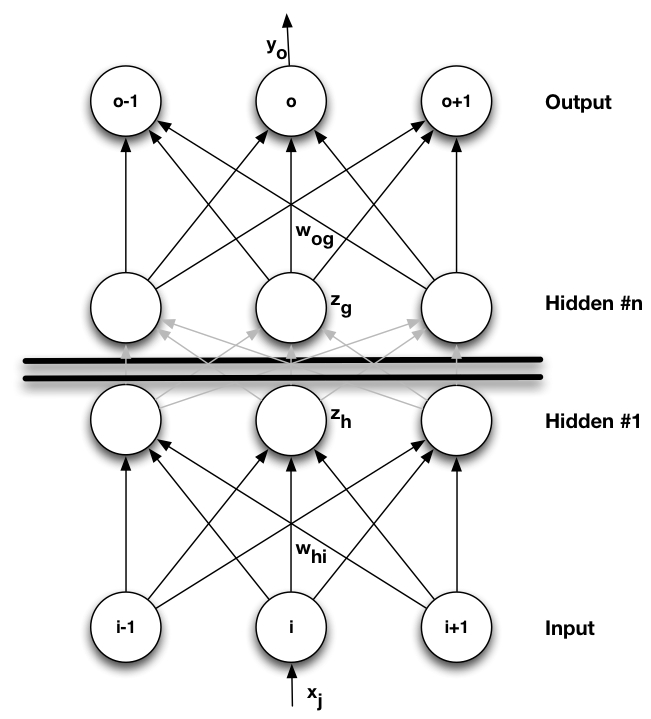
\includegraphics{NeuralNet_InHidOut-full.jpg}
\caption{Layout of \textit{Multilayer Perceptron}.}
\label{NeuralNet_InHidHidOut_full}
\end{center}
\end{figure}

Each nod in the lower layer is connected to all nodes in the layer above and a weight is associated with the connection, for example $w_{hi}$ in figure \ref{NeuralNet_InHidHidOut_full}. The output of a node in the network is calculated with a so called activation function which input is the weighted sum of the incoming connections. Activation functions are covered in subsection \ref{sss:activation_function}. A error function is used to calculate the difference between the output from the network and the target (desire) value, this is typically the mean square error function $E = \frac{1}{2} (t - y)^{2} $ but other functions are also used. In this paper the supervised training algorithm called back-propagation is used to create the statistical model. This algorithm can briefly be described as follows:
\
\begin{enumerate}
\item Sample from the training set is presented (indata to input nodes).
\item Inputs are propagated forward in the network by calculating output values for the nodes in each layer by applying the activation function from input nodes towards output node. \textit{Forward propagation}
\item Output error is calculated by the error function $ E = \frac{1}{2} (t - y)^{2} $. Here $t$ is the target value and $y$ is the output of the network. 
\item \textit{Backward propagation}
\item Calculate the gradient, momentum ($ M(t) = M(t-1) * \lambda - \textit{gradient}$) and update weights ($ W(t) = \alpha * M(t)$), here $\lambda$ = velocity decay, $\alpha$ = learning rate.
\end{enumerate} 
The algorithm described above is applied on the whole testdata set and repeated for the desired number of iterations. At this point all weights are adjusted to represent a god model of the problem. Initialization of the weights are discussed in subsection \ref{sss:weight_bias_initialization}. 
\
Three different regimes of weight updates are often used:
\begin{itemize}
\item \textit{Online}. Weights are updated after every sample in the test dataset. 
\item \textit{Batch}. Weights are updated after passing all training data.
\item \textit{Mini-batch}. Divide the training data set into chunks of equal size and update the weights after passing a chunk.
\end{itemize} 
The selected regime of weight update foremost affects the speed of the learning. In subsection \ref{sss:boosting_mlp_minibatch} the speed gain of using the mini-batch versus batch regime is explored. In some situations the learning algorithm can give rise to so called overfitting which leads to less favourable predictions for the verification set. Overfitting can be avoided by adding noise to the weights, this is future elaborated in subsection \ref{sss:dropout_regime}.
\
The first assessment was to use Weka as the major platform for testing and building models. However it was soon clear that the performance of the platform was to poor to offer a workable environment. Though Weka was used to get a feel of the dataset, test out MLP configurations and perform a principal component analyse. Several MLP configurations were tested and evaluated to gather basic data. The sigmoid activation function was not able to create good models so Weka was supplemented with a hyperbolic tangent function, which outperformed the sigmoid networks and produced good models.  

%***
%* Activation function
%***
\subsubsection{Activation function} \label{sss:activation_function}
\texttt{ToDo: More stuff...}

%***
%* 
%***
%\subsubsection{Cost function}

%***
%* Weight and bias initialization
%***
\subsubsection{Weight and bias initialization} \label{sss:weight_bias_initialization}

\begin{equation} \label{eq:weight_init_regular}
W_{ij} \sim U[-\frac{1}{\sqrt{n_{i-1}}},\frac{1}{\sqrt{n_{i-1}}}]
\end{equation}

normalized initialization
\begin{equation} \label{eq:weight_init_normalized}
W_{ij} \sim U[-\frac{\sqrt{6}}{\sqrt{n_{i-1}+n_{i}}},\frac{\sqrt{6}}{\sqrt{n_{i-1}+n_{i}}}]
\end{equation}

where U[-x,x] is the uniform distribution in the interval $-x < a < x$ and $n_{i}$ is the number of nodes in layer i.

%***
%* Weight update regime
%***
\subsubsection{Weight update regime} \label{sss:weight_regime}
Multilayer perceptron models can with advantage be built with use of the Backpropagation algorithm and have Gradient Descent as one of its corner stones. Choosing a good regime of weight updating is there for crucial. It is more rewarding to follow small but consistent gradients when updating the weights then bigger and more inconsistent ones. In this paper we use two mechanisms to refine the process of updating the weight: learning rate and momentum. 
The concept of adding learning rate can be viewed as a way to control how fast the weights should be learned in a update. For data sets with redundant data the learning rate can be low thou to low learning rate will slow down the learning considerable, to high rate can make the learning overshoot. It is often favourable to keep the learning rate high in the beginning and turning it down further along in the update process.   
\\
The method of using momentum steams from the idea of adding a momentum to the current gradient in the gradient decent algorithm rather then follow the steepest decent. Adding a momentum based on the previous weight updates to the current gradient makes it keep going in the previous direction, a momentum, see equation \ref{eq:wupdate_first}. 

\begin{equation} \label{eq:wupdate_first}
 \mathbf{v}_{t} = \alpha \mathbf{v}_{t-1} - \epsilon \frac{\partial{E_{t}}}{\partial{\mathbf{w}_{t}}} 
\end{equation}

\begin{equation} \label{eq:wupdate_eq}
\Delta \mathbf{w}_{t} = \mathbf{v}_{t} 
\end{equation}

\begin{equation} \label{eq:wupdate_final}
\Delta \mathbf{w}_{t} = \alpha \Delta \mathbf{w}_{t-1} - \epsilon \frac{\partial{E_{t}}}{\partial{\mathbf{w}_{t}}} 
\end{equation}
Weight update can be expressed in terms of the velocity, see equation \ref{eq:wupdate_eq}. Expressing the update in terms of previous weight update gives the equation \ref{eq:wupdate_final}. This combined with the learning rate gives the final update function $\lambda \Delta \mathbf{w}_{t}$ where $\lambda$ is the learning rate and $\alpha$ the momentum multiplier.


%***
%* Dropout regime
%***
\subsubsection{Dropout regime} \label{sss:dropout_regime}
\texttt{ToDo: More stuff...}


%========================================
%===
%=== Optimization with Genetic Algorithm 
%===
%========================================
\subsection{Optimization with Genetic Algorithm}
\texttt{ToDo: More stuff...}

%***
%* Genome
%***
\subsubsection{Genome}
\texttt{ToDo: More stuff...}

%***
%* Objective function
%***
\subsubsection{Objective function}
\texttt{ToDo: More stuff...}

%***
%* Crossover and mutation
%***
\subsubsection{Crossover and mutation}
\texttt{ToDo: More stuff...}

%***
%* The search process
%***
\subsubsection{The search process}
\texttt{ToDo: More stuff...}





\pagebreak
\section{The mathematics of Backpropagation}

%\documentclass[a4paper]{article}
%
%\author{Rasmus Tibell}
%\title{Master Thesis Example}
%
%\usepackage{graphicx}
%\usepackage{multirow}
%\usepackage{mathtools}
%\begin{document}


%\section{The mathematics behind the Multi\-layer Perseptron}
The model consists of L feature variables, this is the same number as input neurons, figure  \ref{NeuralNet_InHidHidOut} shows the configuration of the network.
Each record in the training data is comprised of the feature variables $\textbf{x} =\{x_{(1)}, x_{(2)}, \ldots , x_{(L)}\}$
 and a target variable y. The training set consists of M tuples as follows: 
 $\textbf{T} =\{(x^{(1)}, y^{(1)}), (x^{(2)}, y^{(2)}), \ldots , (x^{(M)}, y^{(M)})\}$


\subsection{Layout of the neural netowork}
This paper will mainly cover multilayer perseptrons with input nodes, one or two hidden layers and a regression output node. Note that only regression output will be used so the output unit is linear and no Softmax will be included. 

\begin{figure}[h!] 
\begin{center}
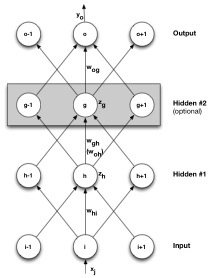
\includegraphics{NeuralNet_InHidOut.jpg}
\caption{Layout of \textit{neural network}. Note that the hidden layer in the lower part of the figure are optional, both network with one and two hidden layers will be discussed.}
\label{NeuralNet_InHidHidOut}
\end{center}
\end{figure}

Let I denote the number of output neurons and H,G the number of hidden units, see figure \ref{NeuralNet_InHidHidOut}. Finaly the number of input neurons are given by L.


\subsection{Error function}
The error function is used to measure the error between the actual value and the prediction. Define the error function E (equation \ref{eq:error_function}) as the sum of the squared differances between the expected and calculated output , $n \in trainingset$. Nota bene that the erorr function for the regression case is different from the functioin used with classification.
\begin{equation} \label{eq:error_function}
E = \frac{1}{2} \sum_{n}{(t^{(n)}-y^{(n)})^{2}}
\end{equation}

Taking the derivative of E (equation \ref{eq:error_function}) with respect to the weights gives us the following function:

\begin{equation} \label{eq:error_function_part_w} 
\frac{\partial{E}}{\partial{w_{i}}} = \frac{1}{2} \sum_{n}{\frac{\partial{y^{(n)}}}{\partial{w_{i}}} \frac{\partial{E}}{\partial{y^{(n)}}}} = -\sum_{n}{\frac{\partial{y^{(n)}}}{\partial{w_{i}}}(t^{(n)}-y^{(n)})}
\end{equation}
\\
We can now form the batch delta rule $\Delta w_{i}$ as
\begin{equation} \label{eq:batch_delta_rule}
\Delta w_{i} = -\epsilon \frac{\partial{E}}{\partial{w_{i}}} = \sum_{n}{\epsilon \frac{\partial{y^{(n)}}}{\partial{w_{i}}}(t^{(n)}-y^{(n)})}
\end{equation}




\subsection{Activation functions in the nodes}
ToDo
\subsubsection{Output neuron (Linear)}
The linear neurons activation function is defined as
\begin{equation} \label{eq:linj_func}
y = \sum_{i}x_{i}w_{i} 
\end{equation} 
\\
The partial derivatives of the linear activation function are
\begin{equation} \label{eq:linear_partial_w}
\frac{\partial{y}}{\partial{w_{i}}} = x_{i}
\end{equation}
and
\begin{equation} \label{eq:linear_partial_x}
\frac{\partial{y}}{\partial{x_{i}}} = w_{i}
\end{equation}

\subsubsection{Logistic neuron (Sigmoid)}
Define the activation function for the logistic neuron as
\begin{equation} \label{eq:sigmoid_func}
y = \frac{1}{1+e^{-z}} 
\end{equation}  
where 
\begin{equation} \label{eq:sigmoid_func_z}
 z = b+\sum_{i}x_{i}w_{i}
\end{equation}  
\\
The derivative of y is $\frac{dy}{dz} = y(1-y)$
\\
Partial derivatives for z are $\frac{\partial{z}}{\partial{w_{i}}} = x_{i}$ and $\frac{\partial{z}}{\partial{x_{i}}} = w_{i}$. Now can the partial derivative of y with respect to $w_{i}$ be defined
\begin{equation} \label{eq:sigmoid_partial_w}
\frac{\partial{y}}{\partial{w_{i}}} =\frac{\partial{y}}{\partial{z}}\frac{\partial{z}}{\partial{w_{i}}} = y(1-y)x_{i}
\end{equation}

\subsubsection{Hyperbolig tangent neuron}
Hyperbolic neuron is defined as
\begin{equation} \label{eq:tanh_func}
y = \frac{e^{z}-e^{-z}}{e^{z}+e^{-z}}
\end{equation}
where 
\begin{equation} \label{eq:tanh_func_z}
z = b+\sum_{i}x_{i}w_{i} 
\end{equation} 
\\
The derivative of y is $\frac{dy}{dz} = (1+y)(1-y)$
\\
Partial derivatives for z are $\frac{\partial{z}}{\partial{w_{i}}} = x_{i}$ and $\frac{\partial{z}}{\partial{x_{i}}} = w_{i}$. From this follows the partial derivative of y with respect to $w_{i}$ is
\begin{equation} \label{eq:tanh_partial_w}
\frac{\partial{y}}{\partial{w_{i}}} =\frac{\partial{y}}{\partial{z}}\frac{\partial{z}}{\partial{w_{i}}} = (1+y)(1-y)x_{i}
\end{equation}
and that the partial derivative of y with respect to $x_{i}$ is
\begin{equation} \label{eq:tanh_partial_x}
\frac{\partial{y}}{\partial{x_{i}}} =\frac{\partial{y}}{\partial{z}}\frac{\partial{z}}{\partial{x_{i}}} = (1+y)(1-y)w_{i}
\end{equation}


\subsection{Finding the gradiants for the error function}
In this section the gradient for the error function both for multilayer perceptrons with singe and dual layers of hidden units is defined. The notations is based on the network configuration shown in figure \ref{NeuralNet_InHidHidOut}.

\subsubsection{Single hidden layer with hyperbolic activation function} \label{ch:single_hidden_layer}
We need to find $\frac{\partial{E}}{\partial{w_{oh}}}$ and $\frac{\partial{E}}{\partial{w_{hi}}}$ in order to performe the calcualtions required by the back propagation algorithm. As before $\epsilon$ is the lerning of the gradient decent. We use $\Delta w_{oh}$ and $\Delta w_{hi} $ to update the wights $w_{oh}$ and $w_{hi}$ respectivly. 
N is the number of observations in a minibatch and $n \in minibatch$.

For the first weight between the output node and the hidden unit we need to calculate $\Delta w_{oh}$.

\begin{equation} \label{eq:gen_error_d_weight_oh}
\Delta w_{oh} = \epsilon \frac{\partial{E}}{\partial{w_{oh}}} = \epsilon \frac{\partial{E}}{\partial{y^{(n)}_{o}}} \frac{\partial{y^{(n)}_{o}}}{\partial{w_{oh}}}
\end{equation}

From equation (\ref{eq:error_function_part_w}) we get $\frac{\partial{E}}{\partial{y}}$
and from equation (\ref{eq:linear_partial_w}) we get $\frac{\partial{y}}{\partial{w_{oh}}}$.
This gives us the solution for equation (\ref{eq:gen_error_d_weight_oh}) as
\begin{equation} \label{eq:gen_error_d_weight_oh_final}
\Delta w_{oh}  = \epsilon \sum_{n} (t^{(n)_{o}}-y^{(n)}_{o}) z^{(n)}_{h} 
\end{equation}

The delta for the weigths between the input node and the hidden layer is given by $\Delta w_{hi} $. 

\begin{equation} \label{eq:gen_error_d_weight_hi}
\Delta w_{hi} = \epsilon \frac{\partial{E}}{\partial{w_{hi}}} = \epsilon \frac{\partial{E}}{\partial{y^{(n)}_{o}}} \frac{\partial{y^{(n)}_{o}}}{\partial{z^{(n)}_{h}}} \frac{\partial{z^{(n)}_{h}}}{\partial{w_{hi}}}
\end{equation}
From equation (\ref{eq:error_function_part_w}) we get $\frac{\partial{E}}{\partial{y}}$
and from equation (\ref{eq:linear_partial_x}) we get $\frac{\partial{y}}{\partial{z_{h}}}$.
The final part $\frac{\partial{z_{h}}}{\partial{w_{hi}}}$ can we obtain from equation (\ref{eq:tanh_partial_w}). This gives us sulution for equation (\ref{eq:gen_error_d_weight_hi}) as
\begin{multline} \label{eq:gen_error_d_weight_hi_final}
\Delta w_{hi}  = \epsilon \frac{\partial{E}}{\partial{y^{(n)}_{o}}} \frac{\partial{y^{(n)}_{o}}}{\partial{z^{(n)}_{h}}} \frac{\partial{z^{(n)}_{h}}}{\partial{w_{hi}}} = \\
\epsilon \sum_{n} \sum_{o}(t^{(n)}_{o}-y^{(n)}_{o}) w_{oh} (1+z^{(n)}_{h})(1-z^{(n)}_{h}) x^{(n)}_{i}
\end{multline}




\subsubsection{Dual hidden layers with hyperbolic activation function} \label{ch:dual_hidden_layer}
For the dual hidden layer configuration we are going to use the two delta wights $\frac{\partial{E}}{\partial{w_{og}}}$ (previously named $\frac{\partial{E}}{\partial{w_{oh}}}$) and $\frac{\partial{E}}{\partial{w_{gh}}}$ (previously named $\frac{\partial{E}}{\partial{w_{hi}}}$) from previous section \ref{ch:single_hidden_layer} and one aditional weight between the input nodes and lower hidden layer $\frac{\partial{E}}{\partial{w_{hi}}}$, for the notations see figure \ref{NeuralNet_InHidHidOut}.
\\
The delta for the weights between the output units and the upper hidden layer, $\Delta w_{og}$ is given by equation ($\ref{eq:gen_error_d_weight_oh}$) but with the indexes renamed. 
\begin{equation} \label{eq:gen_dual_error_d_weight_og}
\Delta w_{og} = 
\epsilon \frac{\partial{E}}{\partial{w_{og}}} = 
\epsilon \frac{\partial{E}}{\partial{y^{(n)}_{o}}} \frac{\partial{y^{(n)}_{o}}}{\partial{w_{og}}} = 
\epsilon \sum_{n} (t^{(n)}_{o}-y^{(n)}_{o}) z^{(n)}_{g}
\end{equation}


The same holds for the delta weights between the two hidden layers $\Delta w_{gh}$ that can be obtained by rewriting the indexes of equation ($\ref{eq:gen_error_d_weight_hi}$) with the indexes renamed. 

\begin{multline} \label{eq:gen_dual_error_d_weight_gh}
\Delta w_{gh} = 
\epsilon \frac{\partial{E}}{\partial{w_{gh}}} = 
\epsilon \frac{\partial{E}}{\partial{y^{(n)}_{o}}} \frac{\partial{y^{(n)}_{o}}}{\partial{z^{(n)}_{g}}} \frac{\partial{z^{(n)}_{g}}}{\partial{w_{gh}}} = \\
\epsilon \sum_{n} \sum_{o}(t^{(n)}_{o}-y^{(n)}_{o}) w_{og} (1+z^{(n)}_{g})(1-z^{(n)}_{g}) z^{(n)}_{h}
\end{multline}

For the final delta weight  $\Delta w_{hi}$ we have to perform some additional work to solve the equation. We need to find the partial derivative $\frac{\partial{z^{(n)}_{g}}}{\partial{z^{(n)}_{h}}}$. Using the equation ($\ref{eq:tanh_partial_x}$) we can get
\begin{displaymath}
\frac{\partial{z^{(n)}_{g}}}{\partial{z^{(n)}_{h}}} = (1+z^{(n)}_{g})(1-z^{(n)}_{g}) w_{gh}
\end{displaymath}

Now we can find the equation for $\Delta w_{hi}$ using the above partial derivative
\begin{multline} \label{eq:gen_dual_error_d_weight_hi_final}
\Delta w_{hi}  = 
\epsilon \frac{\partial{E}}{\partial{w_{hi}}} = 
\epsilon \frac{\partial{E}}{\partial{y^{(n)}_{o}}} \frac{\partial{y^{(n)}_{o}}}{\partial{z^{(n)}_{g}}} \frac{\partial{z^{(n)}_{g}}}{\partial{z^{(n)}_{h}}} \frac{\partial{z^{(n)}_{h}}}{\partial{w_{hi}}} = \\
\epsilon \sum_{n} \sum_{o} \sum_{g} (t^{(n)}_{o}-y^{(n)}_{o}) w_{og} (1+z^{(n)}_{g})(1-z^{(n)}_{g}) w_{gh} (1+z^{(n)}_{h})(1-z^{(n)}_{h}) x^{(n)}_{i}
\end{multline}





\subsection{Matrix calculations for the MLP}
Let $H_{1}$ and $H_{2}$ be the number of hidden units for layer 1 and 2. The number of inputs are represented by $I$ and the number of observation in a minibatch is $N$. For regression output, as in this paper the number of output units is equal to one and is denoted by $O$.  

Let $\mathbf{X}$ be a $I \times N$ matrix of the input features in a minibatch, $\mathbf{Y}$ and $\mathbf{T}$ are matrices of size $O \times N$ and denotes the predicted value and target value respectively. 

\subsubsection{Single hidden layer with hyperbolic activation function} \label{ch:mtx_single_hidden_layer}
 Let $\mathbf{\Theta}$ be the $O \times H_{1}$ matrix of weights on the connection from hidden units to output units and $\mathbf{W}$ is the $I \times H_{1}$ matrix with weights on the connections from input units to the hidden units. The output of the hidden unit is represented as a $H_{1} \times N$ matrix $\mathbf{\Psi}$ for a single minibatch.  
 \\
 Now we can represent the equation (\ref{eq:gen_error_d_weight_oh_final}) in vectorized form as
\begin{displaymath}
 \frac{1}{N}(\mathbf{Y}-\mathbf{T}) \mathbf{\Psi^{T}} 
 \end{displaymath}
 \\
 and for equation (\ref{eq:gen_error_d_weight_hi_final}) we get
 \begin{displaymath}
 \frac{1}{N}(\mathbf{\Theta^{T}}(\mathbf{Y}-\mathbf{T})) \circ (\mathbf{1} - \mathbf{\Psi}) \circ (\mathbf{1} - \mathbf{\Psi}) \mathbf{X^{T}}
 \end{displaymath}

\subsubsection{Dual hidden layers with hyperbolic activation function} \label{ch:mtx_dual_hidden_layer}
Now let $\mathbf{\Theta}$ be the $O \times H_{2}$ matrix of weights on the connection from the second layer of hidden units to output units and $\mathbf{W}$ is the $I \times H_{1}$ matrix with weights on the connections from input units to the first layer of hidden units. The output of the first hidden unit is represented as a $H_{1} \times N$ matrix $\mathbf{\Upsilon}$ and a $H_{2} \times N$ matrix $\mathbf{\Psi}$ for the second layer.
Let $\mathbf{\Xi}$ be the $H_{1} \times H_{2}$ matrix of weights on the connections between the hidden layers.
\\
 Now we can represent the equation (\ref{eq:gen_dual_error_d_weight_og}) in vectorized form as
\begin{displaymath}
 \frac{1}{N}(\mathbf{Y}-\mathbf{T}) \mathbf{\Psi^{T}} 
 \end{displaymath}
 \\
 and for equation (\ref{eq:gen_dual_error_d_weight_gh}) we get
 \begin{displaymath}
 \frac{1}{N}(\mathbf{\Theta^{T}}(\mathbf{Y}-\mathbf{T})) \circ (\mathbf{1} - \mathbf{\Psi}) \circ (\mathbf{1} - \mathbf{\Psi}) \mathbf{\Upsilon^{T}}
 \end{displaymath}
  and finaly for equation (\ref{eq:gen_dual_error_d_weight_hi_final}) we get
\begin{displaymath}
 \frac{1}{N}\Xi((\mathbf{\Theta^{T}}(\mathbf{Y}-\mathbf{T})) \circ (\mathbf{1} - \mathbf{\Psi}) \circ (\mathbf{1} + \mathbf{\Psi})) \circ
 (\mathbf{1} - \mathbf{\Upsilon}) \circ (\mathbf{1} + \mathbf{\Upsilon}) \mathbf{X^{T}}
 \end{displaymath}

If we take the weight decay into account the final matrix representation for equations (\ref{eq:gen_dual_error_d_weight_og}, \ref{eq:gen_dual_error_d_weight_gh}, \ref{eq:gen_dual_error_d_weight_hi_final}) becomes
\begin{displaymath}
\frac{1}{N}(\mathbf{Y}-\mathbf{T}) \mathbf{\Psi^{T}} + \lambda \Theta
 \end{displaymath}
 \begin{displaymath}
 \frac{1}{N}(\mathbf{\Theta^{T}}(\mathbf{Y}-\mathbf{T})) \circ (\mathbf{1} - \mathbf{\Psi}) \circ (\mathbf{1} - \mathbf{\Psi}) \mathbf{\Upsilon^{T}} + \lambda \Xi
\end{displaymath}
\begin{displaymath}
\frac{1}{N}\Xi((\mathbf{\Theta^{T}}(\mathbf{Y}-\mathbf{T})) \circ (\mathbf{1} - \mathbf{\Psi}) \circ (\mathbf{1} + \mathbf{\Psi})) \circ
 (\mathbf{1} - \mathbf{\Upsilon}) \circ (\mathbf{1} + \mathbf{\Upsilon}) \mathbf{X^{T}} - \lambda W
 \end{displaymath}
\\
Where $\circ$ is the element-wise multiplication operator.

%\end{document}




\section{Experiments and Results} \label{ss:results}
\texttt{ToDo: Describe the results of the experiments}

%========================================
%===
%=== Principal components analyse (PCA)
%===
%========================================
\subsection{Principal components analyse (PCA)} \label{sss:pca_analyse}
\texttt{ToDo: Describe and document the experiments with PCA}

%========================================
%===
%=== Performance of support vector regression (SVR)
%===
%========================================
\subsection{Performance of support vector regression (SVR)} \label{sss:performance_svr}
Performance of the Multilayer Perceptron is compared against a more commonly used machine learning algorithm, the support vector regression algorithm was chosen as a basis for this comparisons. Henceforth the Support Vector Machine and Support Vector Regression will be shortened to SVM and SVR respectively. Tests of the SVR performance is based on the open source library Libsvm using the Python implementation. Calculations is done using the epsilon-SVM which uses the epsilon intensive loss function. Common parameters used by the SVR are: $\epsilon$ (epsilon) used in the loss function and the cost parameter C.
To give the SVR model a fair chance three different kernels were evaluated: Radial, Sigmoid and Polynomial. These test runs are described in the tables \ref{tab:params_svr_radial}, \ref{tab:params_svr_sigmoid} and \ref{tab:params_svr_poly} of the following subsections. Two different methods of finding the parameters were used, one with manually selected parameters and the other using a genetic algorithm. In the first approach parameter ranges were selected manually in an initial run and with knowledge from that stage a second run was performed with narrowed parameter intervals. Each parameter where tested with about 4-5 points in the interval. The second approach was to let a genetic algorithm select the best parameter set, this procedure is described in details in subsection \ref{sss:ga_tuning}.  

%***
%* Radial Kernel
%***
\subsubsection{Radial Kernel} \label{sss:performance_radial_svr}
The Radial kernel is calculated using the radial basis function (RBF) $e^{-\gamma|u-v|^{2}}$. One kernel parameter $\gamma$ is used.

\begin{table}[H]
\begin{threeparttable}
\begin{tabular}{ | l | l | l | l | l | l | } 
\hline 
Kernel & Run & Param & Low & Hi & Best \\
\hline 
\multirow{21}{*}{Radial} % $e^{-\gamma|u-v|^{2}}$}
& \multirow{7}{*}{Course} & Cost param & 2 & 512 & 256 \\
& & Kernel gamma & 3,051758e-05 & 1,0 & 0,015625 \\  
& & Loss epsilon & 0,000244 & 1,0 & 0,015625 \\ 
\cline{3-6}
& & \multirow{2}{*}{Verify} & \multicolumn{2}{l|}{Error in \%} & 0,040715 \\
& & & \multicolumn{2}{l|}{RMS error} & 0,055867 \\
\cline{3-6}
& & \multirow{2}{*}{Test} & \multicolumn{2}{l|}{Error in \%} & 0,054865 \\
& & & \multicolumn{2}{l|}{RMS error} & 0,073860 \\
\cline{2-6}
& \multirow{7}{*}{Fine} & Cost param & 2,853117 & 4,594973 & 3,797498 \\
& & Kernel gamma & 0,016600 & 0,751315 & 0,111678 \\  
& & Loss epsilon & 0,002039 & 0,092296 & 0,005289 \\
\cline{3-6}
& & \multirow{2}{*}{Verify} & \multicolumn{2}{l|}{Error in \%} & 0,040370 \\
& & & \multicolumn{2}{l|}{RMS error} & 0,055633 \\
\cline{3-6}
& & \multirow{2}{*}{Test} & \multicolumn{2}{l|}{Error in \%} & 0,056366 \\
& & & \multicolumn{2}{l|}{RMS error} & 0,075934 \\
\cline{2-6}
& \multirow{7}{*}{GA} & Cost param & 0,25 & 64 & 5,75 \\
& & Kernel gamma & 0,031250  & 0,156250 & 0,085449 \\  
& & Loss epsilon & 0,003906 & 0,019531 & 0,008057 \\
\cline{3-6}
& & \multirow{2}{*}{Verify} & \multicolumn{2}{l|}{Error in \%} & 0,040241 \\
& & & \multicolumn{2}{l|}{RMS error} & 0,055460 \\
\cline{3-6}
& & \multirow{2}{*}{Test} & \multicolumn{2}{l|}{Error in \%} & 0,056041 \\
& & & \multicolumn{2}{l|}{RMS error} & 0,075436 \\
\hline
\end{tabular}
\begin{tablenotes}
      \small
      \item Radial: $e^{-\gamma|u-v|^{2}}$, GA: population=200, generations=100, selection=50\% X-over=50\%, mutation=5\%
\end{tablenotes}
\caption{Finding parameters for Radial SVR}
\label{tab:params_svr_radial}
\end{threeparttable}
\end{table}


From the table \ref{tab:params_svr_radial} it follows that the lowest verification error are produced by the GA selected parameters giving a RMS error of 0,055460. Applying the test data on this model gives a RMS error of 0,075436 which actually is higher then for the manually selected parameters would have produced.

%***
%* Sigmoid Kernel
%***
\subsubsection{Sigmoid Kernel} \label{sss:performance_sigmoid_svr}
The Sigmoid kernel is calculated using the equation $tanh(\gamma u^{T} v + c_{0})$. Parameters for this kernel are $\gamma$ and the coefficient $c_{0}$.

\begin{table}[H]
\begin{threeparttable}
\begin{tabular}{ | l | l | l | l | l | l | } 
\hline 
Kernel & Run & Param & Low & Hi & Best \\
\hline 
\multirow{24}{*}{Sigmoid} % $tanh(\gamma u^{T} v + c_{0})$}
& \multirow{8}{*}{Course} & Cost param & 789,75 & 1024 & 1024 \\
& & Kernel gamma & 0,000188 & 8 & 0,000244 \\  
& & $coef_{0}$ & 0,001266 & 1 & 0,001953 \\
& & Loss epsilon & 0,013719 & 1 & 0,015625 \\ 
\cline{3-6}
& & \multirow{2}{*}{Verify} & \multicolumn{2}{l|}{Error in \%} & 0,0466276 \\
& & & \multicolumn{2}{l|}{RMS error} & 0,063818 \\
\cline{3-6}
& & \multirow{2}{*}{Test} & \multicolumn{2}{l|}{Error in \%} & 0,062559 \\
& & & \multicolumn{2}{l|}{RMS error} & 0,084042 \\
\cline{2-6}
& \multirow{8}{*}{Fine} & Cost param & 955,59 & 1692,89 & 1692,89 \\
& & Kernel gamma & 0,000367 & 0,000590 & 0,000537 \\  
& & $coef_{0}$ & 0,000865 & 0,001532 & 0,001266 \\
& & Loss epsilon & 0,022095 & 0,032349 & 0,022095 \\
\cline{3-6}
& & \multirow{2}{*}{Verify} & \multicolumn{2}{l|}{Error in \%} & 0,045878 \\
& & & \multicolumn{2}{l|}{RMS error} & 0,062007 \\
\cline{3-6}
& & \multirow{2}{*}{Test} & \multicolumn{2}{l|}{Error in \%} & 0,062063 \\
& & & \multicolumn{2}{l|}{RMS error} & 0,082555 \\
\cline{2-6}
& \multirow{8}{*}{GA} & Cost param & 0,03125 & 7,9688 & 7,8750 \\
& & Kernel gamma & 0,01562 & 1,01562 & 0,01562 \\  
& & $coef_{0}$ & -0,5 & 0,5 & -0,50000 \\
& & Loss epsilon & 0,00098 & 1,0010 & 0,02344 \\ 
\cline{3-6}
& & \multirow{2}{*}{Verify} & \multicolumn{2}{l|}{Error in \%} & 0,044256 \\
& & & \multicolumn{2}{l|}{RMS error} & 0,060323 \\
\cline{3-6}
& & \multirow{2}{*}{Test} & \multicolumn{2}{l|}{Error in \%} & 0,058019 \\
& & & \multicolumn{2}{l|}{RMS error} & 0,078112 \\
\hline
\end{tabular}
\begin{tablenotes}
      \small
      \item Sigmoid: $tanh(\gamma u^{T} v + c_{0})$, GA: population=200, generations=100, selection=50\% X-over=50\%, mutation=5\%
\end{tablenotes}
\caption{Finding parameters for Sigmoid SVR}
\label{tab:params_svr_sigmoid}
\end{threeparttable}
\end{table}

Results from the Sigmoid kernel is obtained in the table \ref{tab:params_svr_sigmoid}. For this kernel the best results, based on the RMS error, are obtained for the model with parameters picked by the GA, with an RMS error of 0,060323 for the verification set and 0,078112 for the test set. This is also the over all lowest error rate. 

%***
%* Polynomial Kernel
%***
\subsubsection{Polynomial Kernel} \label{sss:performance_poly_svr}
For the polynomial kernel the kernel function are; $(\gamma u^{T} v + c_{0})^{d}$. This kernel uses tree parameters: $\gamma$ and the coefficient $c_{0}$ as for the Sigmoid kernel in subsection \ref{sss:performance_sigmoid_svr} and with a additional parameter determining the polynomial degree.

\begin{table}[H]
\begin{threeparttable}
\begin{tabular}{ | l | l | l | l | l | l | } 
\hline 
Kernel & Run & Param & Low & Hi & Best \\
\hline 
\multirow{24}{*}{Poly} % $(\gamma u^{T} v + c_{0})^{d}$}
& \multirow{8}{*}{Course} & Cost param & 0,015625 & 16 & 0,5 \\
& & Kernel gamma & 0,003906 & 0,25 & 0,03125 \\  
& & Kernal degree & 2 & 8 & 8 \\
& & Loss epsilon & 0,007812 & 0,125 & 0,007812 \\ 
\cline{3-6}
& & \multirow{2}{*}{Verify} & \multicolumn{2}{l|}{Error in \%} & 0,0411920 \\
& & & \multicolumn{2}{l|}{RMS error} & 0,0560074 \\
\cline{3-6}
& & \multirow{2}{*}{Test} & \multicolumn{2}{l|}{Error in \%} & 0,0579445 \\
& & & \multicolumn{2}{l|}{RMS error} & 0,077401 \\
\cline{2-6}
& \multirow{8}{*}{Fine} & Cost param & 0,31863 & 1,0 & 0,683013 \\
& & Kernel gamma & 0,022095 & 0,385543 & 0,057309 \\  
& & Kernal degree & 2 & 8 & 5 \\
& & Loss epsilon & 0,003284 & 0,239392 & 0,003284 \\
\cline{3-6}
& & \multirow{2}{*}{Verify} & \multicolumn{2}{l|}{Error in \%} & 0,040356 \\
& & & \multicolumn{2}{l|}{RMS error} & 0,055638 \\
\cline{3-6}
& & \multirow{2}{*}{Test} & \multicolumn{2}{l|}{Error in \%} & 0,056168 \\
& & & \multicolumn{2}{l|}{RMS error} & 0,075729 \\
\cline{2-6}
& \multirow{8}{*}{GA} & Cost param & 0,001 & 4,984375 & 4,140625 \\
& & Kernel gamma & 0,003906 & 1,0 & 0,09375 \\  
& & Kernal degree & 1 & 5 & 3 \\
& & Loss epsilon & 0,001953 & 0,017578 & 0,010986 \\
\cline{3-6}
& & \multirow{2}{*}{Verify} & \multicolumn{2}{l|}{Error in \%} & 0,040886 \\
& & & \multicolumn{2}{l|}{RMS error} & 0,055898 \\
\cline{3-6}
& & \multirow{2}{*}{Test} & \multicolumn{2}{l|}{Error in \%} & 0,058598 \\
& & & \multicolumn{2}{l|}{RMS error} & 0,078522 \\
\hline
\end{tabular}
\begin{tablenotes}
      \small
      \item Poly: $(\gamma u^{T} v + c_{0})^{d}$, GA: population=200, generations=100, selection=50\% X-over=50\%, mutation=5\%
\end{tablenotes}
\caption{Finding parameters for Polygon SVR}
\label{tab:params_svr_poly}
\end{threeparttable}
\end{table}
Results from the tests are in the table \ref{tab:params_svr_poly} where it can be seen that the preferred model based on the RMS error of the verification set originates from the manually fine tuned parameter setting. This selection gives a model that generates a RMS error of 0,075729 when applying the test set.


%========================================
%===
%=== Tuning parameters for the Multilayer Perseptron
%===
%========================================
\subsection{Tuning parameters for the Multilayer Perseptron} \label{sss:tuning_mlp}
In this subsection the process of finding appropriate values for the parameters controlling the calculations generating the prediction model.  
\texttt{ToDo: More stuff...}

%***
%* Finding values for learning rate and momentum
%***
\subsubsection{Finding values for learning rate and momentum} \label{sss:tuning_mlp_learning_momentum}
The importance of how the weights are updated is stressed in subsection \ref{sss:weight_regime} where we introduce the concepts: learning rate and momentum. Here we study the effect of these parameters on the model and determines favourable values these. During this process the MLP configuration is fixed to use two hidden layers with 10 nods each, weight decay is set to $10^{-6}$. In the initial trial the algorithm is allowed to run for 500 iterations. The parameter space for the two parameters are initially tested with the values {0,1 0,3 0,6 0,9} corresponding to the first row of table \ref{tab:first_param_tuning}. 

\begin{table}[H]
\begin{threeparttable}
\begin{tabular}{ | p{1.6cm} | p{1.6cm} | l | l | l | l | l | l | } 
\hline 
\multicolumn{2}{|c|}{Test interval} & \multicolumn{2}{|c|}{Best test result} & \multicolumn{1}{|c|}{Validation error}  & \multicolumn{1}{|c|}{Test error} \\
\hline 
L-rate & Moment & L-rate & Moment & RMS  & RMS  \\
\hline
0,10 - 0,90 & 0,10 - 0,90 & 0,60 & 0,90 & 0,04537 & 0,04840 \\ %--Source=eval30a
\hline
0,10 - 0,70 & 0,90 - 0,90 & 0,70 & 0,90 & 0,04551 & 0,04843 \\ %--Source=eval30b
\hline
0,60 - 0,70 & 0,85 - 0,95 & 0,675 & 0,95 & 0,04417 & 0,04738 \\ %--Source=eval30c
\hline
0,65 - 0,70 & 0,92 - 0,98 & 0,675 & 0,94 & 0,04440 & 0,04735 \\ %--Source=eval30d
\hline
0,66 - 0,68 & 0,94 - 0,96 & 0,68 & 0,95 & 0,04360 & 0,04686 \\ %--Source=eval20e

%L-rate & Moment & L-rate & Moment & Percent & RMS  & Percent & RMS  \\
%\hline
%0,10 - 0,90 & 0,10 - 0,90 & 0,60 & 0,90 & 0,03167 & 0,04537 & 0,03479 & 0,04840 \\ %--Source=eval30a
%\hline
%0,10 - 0,70 & 0,90 - 0,90 & 0,70 & 0,90 & 0,03168 & 0,04551 & 0,03492 & 0,04843 \\ %--Source=eval30b
%\hline
%0,60 - 0,70 & 0,85 - 0,95 & 0,675 & 0,95 & 0,03074 & 0,04417 & 0,03395 & 0,04738 \\ %--Source=eval30c
%\hline
%0,65 - 0,70 & 0,92 - 0,98 & 0,675 & 0,94 & 0,03067 & 0,04440 & 0,03380 & 0,04735 \\ %--Source=eval30d
%\hline
%0,66 - 0,68 & 0,94 - 0,96 & 0,68 & 0,95 & 0,03025 & 0,04360 & 0,03356 & 0,04686 \\ %--Source=eval20e

\hline
\end{tabular}
\begin{tablenotes}
      \small
      \item Average over 5 runs, weight decay = 1e-6, Nodes = [10,10], Iterations = 500, Mini-batch = 194, no noise added
\end{tablenotes}
\caption{Searching for learning rate and momentum using 500 iterations, averages over 5 runs}
\label{tab:first_param_tuning}
\end{threeparttable}
\end{table}
This test indicates that the best parameter setting is located near a momentum of 0,9 and a learning rate near 0,6. After further testing with parameters in the neighbourhood of the favourable values found in the initial test, the best values for the learning rate is 0,68 and for the momentum it is 0,95. The best results for each test is presented in table \ref{tab:first_param_tuning} and is given as the mean of the results from five runs. 
\\
The previous procedure is repeated using 4000 iterations in order to study the effect on the studied parameters. From these tests it is clear that the learning rate has to be reduced to about 0,30 and with the momentum kept fixed. Increasing the number of iterations favours a lower learning rate that avoids ``overfitting'' the model. Results from these tests are gathered in table \ref{tab:first_param_tuning4k}.  

\begin{table}[H]
\begin{threeparttable}
\begin{tabular}{ | p{1.6cm} | p{1.6cm} | l | l | l | l | l | l | } 
\hline 
\multicolumn{2}{|c|}{Test interval} & \multicolumn{2}{|c|}{Best test result} & \multicolumn{1}{|c|}{Validation error}  & \multicolumn{1}{|c|}{Test error} \\
\hline 
L-rate & Moment & L-rate & Moment & RMS & RMS  \\
\hline
0,10 - 0,90 & 0,10 - 0,90 & 0,30 & 0,90 & 0,04227 & 0,04577 \\ %--Source=eval20a
\hline
0,10 - 0,70 & 0,90 - 0,90 & 0,30 & 0,90 &0,04227 & 0,04579 \\ %--Source=eval20b
\hline
0,10 - 0,30 & 0,85 - 0,95 & 0,30 & 0,95 & 0,04185 & 0,04561 \\ %--Source=eval20c
\hline
0,28 - 0,32 & 0,93 - 0,97 & 0,32 & 0,95 & 0,04190 & 0,04576 \\ %--Source=eval20d
\hline
0,31 - 0,33 & 0,96 - 0,98 & 0,32 & 0,98 & 0,04204 & 0,04567 \\ %--Source=eval20e
\hline
0,30 - 0,50 & 0,90 - 0,99 & 0,30 & 0,95 & 0,04181 & 0,04561 \\ %--Source=eval20f

%L-rate & Moment & L-rate & Moment & Percent & RMS  & Percent & RMS  \\
%\hline
%0,10 - 0,90 & 0,10 - 0,90 & 0,30 & 0,90 & 0,02956 & 0,04227 & 0,03247 & 0,04577 \\ %--Source=eval20a
%\hline
%0,10 - 0,70 & 0,90 - 0,90 & 0,30 & 0,90 & 0,02957 & 0,04227 & 0,03250 & 0,04579 \\ %--Source=eval20b
%\hline
%0,10 - 0,30 & 0,85 - 0,95 & 0,30 & 0,95 & 0,02933 & 0,04185 & 0,03234 & 0,04561 \\ %--Source=eval20c
%\hline
%0,28 - 0,32 & 0,93 - 0,97 & 0,32 & 0,95 & 0,02948 & 0,04190 & 0,03249 & 0,04576 \\ %--Source=eval20d
%\hline
%0,31 - 0,33 & 0,96 - 0,98 & 0,32 & 0,98 & 0,02936 & 0,04204 & 0,03246 & 0,04567 \\ %--Source=eval20e
%\hline
%0,30 - 0,50 & 0,90 - 0,99 & 0,30 & 0,95 & 0,02938 & 0,04181 & 0,03242 & 0,04561 \\ %--Source=eval20f

\hline
\end{tabular}
\begin{tablenotes}
      \small
      \item Average over 5 runs, weight decay = 1e-6, Nodes = [10,10], Iterations = 4000, Mini-batch = 194, no noise added
\end{tablenotes}
\caption{Searching for learning rate and momentum using 4000 iterations, averages over 5 runs}
\label{tab:first_param_tuning4k}
\end{threeparttable}
\end{table}
To close up this subsection we found that the best parameters for a long running algorithm are in the neighbourhood of 0,30 for the learning rate and 0,95 for the momentum. For configurations that uses fever iterations to find a suitable model should use values in the vicinity of 0,68 and 0,95 respectively. 


%***
%* Searching for appropriate MLP configuration
%***
\subsubsection{Searching for appropriate MLP configuration} \label{sss:tuning_mlp_nodeconfig}
Configuration of the network has a profound impact on the models performance. In this work the basic configuration of the network is fixed to four layers: input layer with 54 nodes, one for each feature, two hidden layers with configurable number of nodes for each layer and a single output node producing the regression result. In this subsection the challenge is to find a apposite number of nodes for the internal layers of the network. The initial trials are restricted to sixteen nodes for each of the internal layers, see figure \ref{NeuralNet_InHidHidOut}. For this configuration the best result is obtained for the configuration with 14 nodes in the first hidden layer and 8 in the second. As shown in table \ref{tab:node_L1_L2_tuning} the results are quite unvarying with small difference between the best and worst results for the RMS error for the verification set. The low value for the standard deviation for the best configuration is also a sign of a better consistency among those models.    
 
%(eval21a,b,e)}

\begin{table}[H]
\begin{threeparttable}
\begin{tabular}{ | l | l | l | l | l | l | l | l | l | } 
\hline 
\multicolumn{1}{|c|}{} & \multicolumn{2}{|c|}{Test interval} & \multicolumn{2}{|c|}{Result} & \multicolumn{2}{|c|}{Validation error}  & \multicolumn{2}{|c|}{Test error} \\
\hline 
Type & L1 & L2 & L1 & L2 & RMS & S-dev & RMS & S-dev \\
\hline
%4 - 16 & 4 - 16 & 4 & 16 & 16 & 0,04162 & 0,30e-3 & 0,04580 & 0,14e-3 \\ %-Source=eval21a
%\hline
Best & 4 - 16 & 4 - 16 & 14 & 8 & 0,04167 & 0,19e-3 & 0,04554 & 0,20e-3 \\ %-Source=eval21d
\hline
Worst & 4 - 16 & 4 - 16 & 4 & 14 & 0,04315 & 1,25e-3 & 0,04638 & 0,79e-3 \\ %-Source=eval21d
\hline
%20 - 32 & 16 - 32 & 4 & 32 & 24 &  &  &  &  \\ %-Source=eval21b
%\hline
\end{tabular}
\begin{tablenotes}
      \small
      \item Average over 5 runs, weight decay = 1e-6, learning rate = 0,30, momentum = 0,95, Iterations = 4000, Mini-batch = 194, no noise added, regular init 
      %--Source=eval21
\end{tablenotes}
\caption{Searching for node configuration for L1 and L2, averages over 5 runs}
\label{tab:node_L1_L2_tuning}
\end{threeparttable}
\end{table}

The ability to create a high quality model depends on the number of nodes in the network and number of iterations of the algorithm. Results of this investigation is presented in table \ref{tab:node_L1_L2_tuning_iters} where the search for best node configuration from table \ref{tab:node_L1_L2_tuning} has been performed with five different values for the iteration count. As expected increasing the number of iteration generates models which has lower error rate and produces more homogeneous results.  

%(eval21f,g,h)}

\begin{table}[H]
\begin{threeparttable}
\begin{tabular}{ | l | p{0.7cm} | p{0.7cm} | l | p{1.3cm} | p{1.3cm} | p{1.3cm} | p{1.3cm} | } 
\hline 
\multicolumn{1}{|c|}{} & \multicolumn{2}{|c|}{Best result} & \multicolumn{2}{|c|}{Validation error}  & \multicolumn{2}{|c|}{Test error} \\
\hline 
Iterations & L1 & L2 & RMS & S-dev & RMS & S-dev \\
\hline
125 & 4 & 4 & 0,05745 & 3,92e-3 & 0,05937 & 3,71e-3 \\
\hline
250 & 4 & 16 & 0,04930 & 1,47e-3 & 0,05191 & 1,37e-3 \\
\hline
500 & 12 & 8 & 0,04437 & 0,29e-3 & 0,04772 & 0,39e-3 \\
\hline
750 & 12 & 16 & 0,04327 & 0,55e-3 & 0,04673 & 0,24e-3 \\
\hline
1000 & 12 & 8 & 0,04281 & 0,16e-3 & 0,04609 & 0,49e-3 \\
\hline
\end{tabular}
\begin{tablenotes}
      \small
      \item Average over 5 runs, weight decay = 1e-6, Nodes[4-16,4-16], learning rate = 0,30, momentum = 0,95, Mini-batch = 194, no noise added, regular init 
      %--Source=eval21
\end{tablenotes}
\caption{Impact of iteration length on node configuration for L1 and L2, averages over 5 runs}
\label{tab:node_L1_L2_tuning_iters}
\end{threeparttable}
\end{table}

Further conclusions can be drawn from the results in table \ref{tab:node_L1_L2_tuning_iters} where it shows that models with fewer nodes performs better when the number of iterations is low and contrary for models that are permitted more iterations. This is due to the fact that a more complex MLP requires additional iterations to find a good solution. Each new node contributes to the total dimension of the n-dimensional space to search with gradient descent. 

%========================================
%===
%=== Boosting multilayer perceptron performance
%===
%========================================
\subsection{Boosting multilayer perceptron performance} \label{sss:boosting_mlp}
There are several techniques that can improve the results and speed up the running time of the backpropagation algorithm. In this subsection we discuss early stopping that can prevent over fitting of the model, running time can be improved by the weight update regime called mini-batch. Random initialization of the weights and selection of interval can impact which solution is found by the gradient descent algorithm and in the end affect the quality of the models prediction. Finally the concept of conformal prediction is explored, this algorithm predicts a interval in which the result will stay within the given interval with a parametrized likelihood.   


%***
%* Early stopping
%***
\subsubsection{Early stopping} \label{sss:boosting_mlp_stopping}
Early stopping is a regime intended to reduce the problem of over fitting of the model especial if the network has more nodes then actually required to represent the learning problem. One symptom of this is that the the weights start to move away from 0 particularly for the most important nodes. As the training progresses less important weights are also moving away from 0 the training error decreases but the models ability to generalize is reduced. 

\begin{wrapfigure}{R}{0.6\textwidth}
\vspace{-20pt}
\begin{center}
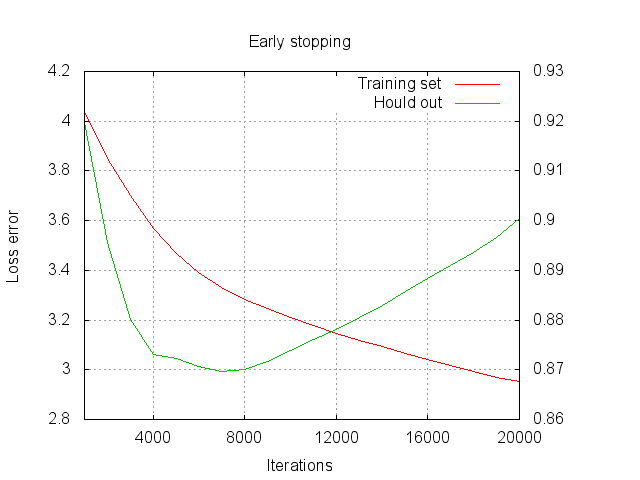
\includegraphics[scale=0.42]{eval24f.png}
\end{center}
\vspace{-20pt}
\caption{Early stopping}
\label{graph:early_stop}
\end{wrapfigure} %-Source=eval24f

The idea behind early stopping is to verify the error rate on a hold out set, in this case the validation set and stop the backpropagation when it increases. This is achieved by monitoring the output of the loss function for the validation data during training. Behaviour of the loss for training and validation sets can be seen in diagram \ref{graph:early_stop}. As long as the loss value decreases the current model are saved and the back propagation continues. If the error on the validation set increases the model are not saved. When the algorithm reaches the predetermined number of iteration the saved model (taken at the lowest seen error rate) is returned as result. So if the error rate decreases asymtotic during the whole backpropagation the final model will be returned if not the intermediary model is used.  
\\

\begin{table}[H]
\begin{threeparttable}
\begin{tabular}{ | l | l | l | l | l | } 
\hline
\multicolumn{1}{|c|}{Testing} & \multicolumn{2}{|c|}{Validation set error}  & \multicolumn{2}{|c|}{Test set error} \\
\hline 
 & Percent & RMS  & Percent & RMS \\
\hline
No early stopping  & 0,03066 & 0,04484 & 0,03306 & 0,04780 \\
\hline
Early stopping & 0,02940 & 0,04154 & 0,03246 & 0,04586 \\
\hline
\end{tabular} 
\begin{tablenotes}
      \small
      \item Average over 5 runs, weight decay = 1e-6, Nodes = [10,10], learning rate = 0,30, momentum = 0,95, Iterations = 50000, Mini-batch = 194, no noise added 
      %--Source=eval124c
\end{tablenotes}
\caption{Early stopping, averages over 5 runns}
\label{tab:early_stop1}
\end{threeparttable}
\end{table}
The result of applying early stopping can be seen in \ref{tab:early_stop1}, here the best result is obtained after about 7000 iterations on average. The favourable effect is significant for both the test and validation set.

%***
%* Mini-batch
%***
\subsubsection{Mini-batch} \label{sss:boosting_mlp_minibatch}
Multilayer Perceptrons can be trained using one of three different schemas discussed in subsection \ref{sss:construction_mlp}. The size of the mini-batch chunks affects the speed of the algorithm, in table \ref{tab:mini_batch1} the algorithm is applied with mini-batch chunks of size 97, 194, 388, 970 and 1940. 

\begin{table}[H]
\begin{threeparttable}
\begin{tabular}{ | l | l | l | l | l | } 
\hline
\multicolumn{1}{|c|}{Testing} & \multicolumn{2}{|c|}{Validation error}  & \multicolumn{2}{|c|}{Runtime} \\
\hline 
Batch size & Percent & RMS error & Running time & Speed up percent\\
\hline
None & 0,02944 & 0,04191 & 159,6 s &  \\
\hline
1940 & 0,02952 & 0,04180 & 129.2 s & 19,0 \\
\hline
970 & 0,02958 & 0,04208 & 91,6 s & 42,6 \\
\hline
388 & 0,02970 & 0,04236 & 81,3 s & 49,0 \\
\hline
194 & 0,02936 & 0,04187 & 78,1 s & 51,0 \\
\hline
97 & 0,02987 & 0,04228 & 75,5 s & 52,7 \\  
\hline
\end{tabular}
\begin{tablenotes}
      \small
      \item Weight decay = 1e-7, Nodes = [10,10], learning rate = 0,30, momentum = 0,95, Iterations = 10000, Early stopping = on, no noise added 
      %--Source=eval25a
\end{tablenotes}
\caption{Mini batch performance, averages over 5 runns}
\label{tab:mini_batch1}
\end{threeparttable}
\end{table}
The rightmost column holds the speed increase of the mini-batch regime over batch processing. As the chunk size of the mini-batch is decreased the root mean square error of the prediction slightly increases due to the fact that fewer samples are used in the calculations that affects the weight update.  

\begin{wrapfigure}{R}{0.6\textwidth}
\vspace{-20pt}
\begin{center}
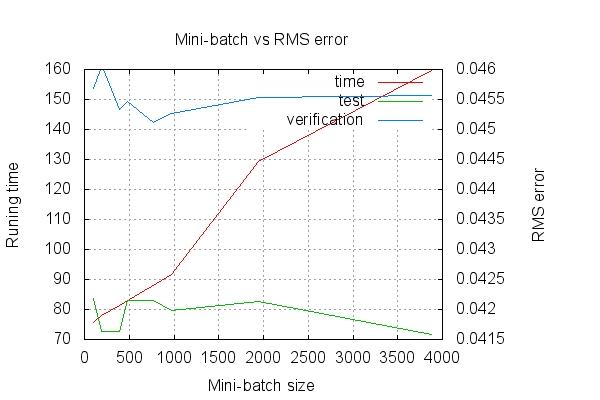
\includegraphics[scale=0.42]{eval25a.png}
\end{center}
\vspace{-20pt}
\caption{Impact of mini-batch size on RMS error}
\label{minibarch_rmsgraph}
\end{wrapfigure}

The results of the tests shows that with a sensible selection of mini-batch chunk size, in this case 970, a good model can be produced in about half the time with a minor increase for the root mean square error.
Studying figure \ref{minibarch_rmsgraph} shows that the RMS error is relatively unaffected by the change of mini-batch size, this behaviour is the same for both the test and verification set. 

\begin{wrapfigure}{R}{0.6\textwidth}
\vspace{-20pt}
\begin{center}
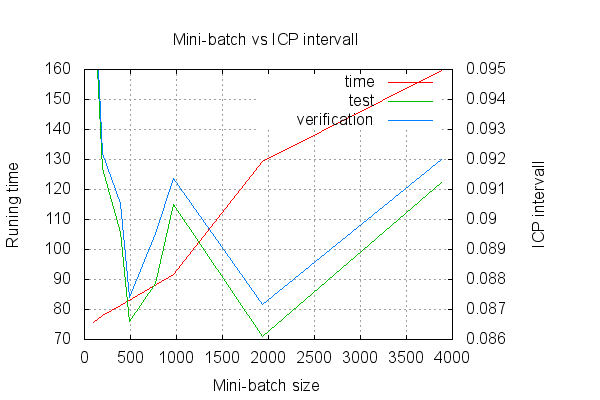
\includegraphics[scale=0.42]{eval25aa.png}
\end{center}
\vspace{-20pt}
\caption{Impact of mini-batch size on ICP-interval}
\label{minibarch_icpgraph}
\end{wrapfigure}

If the ICP interval is taken into account the conditions changes some what. We can see from the figure \ref{minibarch_icpgraph} that a good choice of mini-batch size is 1940 with respect to the performance of the ICP-interval. This gives a speed gain of about 20 percent without increasing the with of the ICP-interval or affects the RMS error significantly. More about the conformal prediction findings in subsection \ref{sss:conformal_prediction}.
\\
In some applications of the MLP processing time is limited due to hardware restrictions or business rules and those gives rise to the mini-batch approach where a good model can be built in a fare amount of time. The total runtime of the model construction can be regulated via the mint-batch size. 


%***
%* Random initialization of weights and dropout
%***
\subsubsection{Random initialization of weights and dropout} \label{sss:boosting_mlp_weight_init}
In this subsection two different schemas for weight initialization are evaluated and the paradigm of ``dropout'' are investigated. 

Initialization of weights are discussed in chapter \ref{sss:glorot_and_bengio} and steams from the work done by Glorot and Bengio in there paper \cite{art}{GlorBeng:10}. The initialization of of the weights is impotent and can have significant effect on the resulting model especial for deep networks. In this work the effect can only be elicited when the noise is added to the weights. When all weights are updated in each iteration the affect of not using the normalized weight initialization is masked by the gradient descent which is still able to find a good solution. This topic is future discussed in chapter \ref{sss:weight_bias_initialization}.

\begin{wrapfigure}{R}{0.6\textwidth}
\vspace{-20pt}
\begin{center}
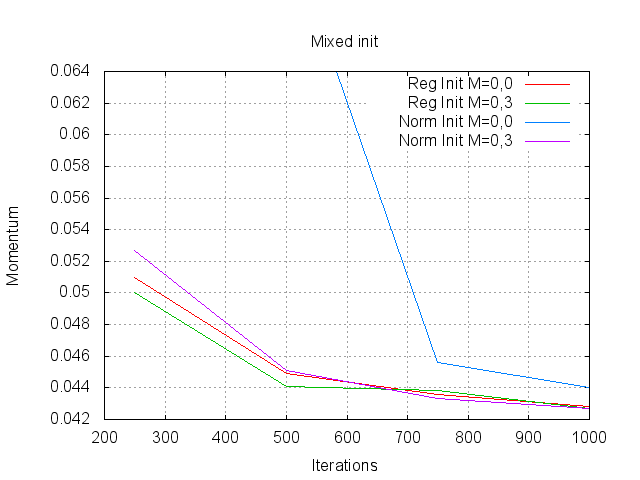
\includegraphics[scale=0.42]{eval33ef.png}
\end{center}
\vspace{-20pt}
\caption{Normalized vs regular initialization}
\label{norm_init}
\end{wrapfigure} %-Source=eval33e, eval33f

The regime of ``dropout'' is discussed in chapter \ref{sss:using_dropout} where the paper \cite{art}{HintSrivKrizSutsSala:12} by Hinton et al. are explored. To investigate the effect five levels of ``dropout'' were tested $\Psi_{M} : M = {0,0 - 0,4}$ (M = proportion of weights left out in weight update), where $\Psi_{0,0}$ corresponds to no ``dropout''.  In diagram \ref{norm_init} the $\Psi_{0,0}, \Psi_{0,3}$ values are presented in conjunction with two weight initialization regimes presented above. From this diagram it can be deduced that ``dropout'' gives an advantage when fewer iteration are used, when the amount of iterations is increased the effect fades out but has clearly a favourable effect for situations where few iteration are used. Future discussions on this topic can be found in chapter \ref{sss:using_dropout}.


%\begin{table}[H]
%begin{threeparttable}
%\begin{tabular}{ | l | l | l | l | l | l | } 
%\hline 
%\multicolumn{2}{|c|}{} & \multicolumn{2}{|c|}{Validation set error}  & \multicolumn{2}{|c|}{Test set error} \\
%\hline 
%Adding noise & Regular init & Percent & RMS  & Percent & RMS \\
%\hline
%\hline
%Yes & Yes & 0,02969 & 0,04226 & 0,03261 & 0,04591 \\
%\hline
%Yes & No & 0,04750 & 0,06595 & 0,05039 & 0,06957 \\
%\hline
%No & Yes & 0,02968 & 0,04216 & 0,03249 & 0,04570 \\
%\hline
%No & No & 0,02998 & 0,04279 & 0,03296 & 0,04652 \\
%\hline
%\end{tabular}
%\begin{tablenotes}
%      \small
%      \item Weight decay = 1e-6, Nodes = 12:6, Iterations = 50000, Early stopping = on, Mini-batch = on, ICP confidence = 95\% 
%      %-Source=eval13b
%\end{tablenotes}
%\caption{Mini batch performance, averages over 4 runns}
%\label{tab:random_initl2}
%\end{threeparttable}
%\end{table}


%***
%* Conformal Prediction
%***
\subsubsection{Conformal Prediction} \label{sss:conformal_prediction}
\texttt{ToDo: More stuff...}

%========================================
%===
%=== Fine tuning of parameters with Genetic Algorithm
%===
%========================================
\subsection{Fine tuning of parameters with Genetic Algorithm} \label{sss:ga_tuning}
Finding appropriate parameters for the Support Vector Regression and the Multilayer Perceptron is a challenge in it self. In article xxxx referred to in xxxx discusses the usage of genetic algorithms to find good parameters. Genetic Algorithms will henceforth often be shortened to GA. The results of the parameter search using a genetic algorithm is presented in the subsection below. A open source package called DEAP (Distributed Evolutionary Algorithms in Python) is used to drive the genetic algorithm in Python. The following parameter configuration was used by the algorithm: a population of 200 individuals running for 100 generations with a selection of 50\%, crossover of 50\%, mutation rate at 5\% and a tournament size of 16. 
\\
\texttt{ToDo: Reference to GA article}

%***
%* Tuning of SVR parameters
%***
\subsubsection{Tuning of SVR parameters} \label{sss:ga_tuning_svr}
The SVR parameters was tuned using a GA previously described. Data from this runns are presented in the tables \ref{tab:params_svr_radial}, \ref{tab:params_svr_sigmoid} and \ref{tab:params_svr_poly} of chapter \ref{sss:performance_svr} and summarised in table \ref{tab:ga_svr_tuning} below.  
\begin{table}[H]
\begin{tabular}{ | l | l | l | l | l |  }
\hline
\multicolumn{1}{|c|}{} & \multicolumn{2}{|c|}{GA tuned} & \multicolumn{2}{|c|}{Manually tuned} \\
\hline
SVR- type & Test error & Test RMS error & Test error & Test RMS error \\
\hline
\hline
Radial & 0,056041 & 0,075436 & 0,056366 & 0,075934 \\
Sigmoid & 0,058019 & 0,078112 & 0,062063 & 0,082555 \\
Polynom & 0,058598 & 0,078522 & 0,056168 & 0,075729 \\
\hline
\end{tabular}
\caption{Tuning of SVR Perseptron using Genetic Algorithm}
\label{tab:ga_svr_tuning}
\end{table}
From the results in table \ref{tab:ga_svr_tuning} it can be seen that no exceptional improvement is gained with the parameters generated using the GA. Performance for the SVR based on a Radial kernel was somewhat better, for the Sigmoid kernel the improvement was the highest in this trial, but the Polynomial kernel performed slightly worse for the model that used GA generated parameters. This vouches for that reasonably good parameters are found and that this results can serve as a good comparison with the results from the MLP. This gives that the MLP has to predict the outcome with a \emph{RMS error below 0,075436} in order to outperform the SVR model. 


%***
%* Tuning of Multilayer Perseptron
%***
\subsubsection{Tuning of Multilayer Perseptron} \label{sss:ga_tuning_mlp}
Inspired from the article \texttt{XXXX} where a GA was used to drive a YYY a GA was constructed to find a good solution to the price estimation problem using a MLP. In this paper we present to different schemas where the optimization is done on two different criteria's. Initially we constructed a GA which goal was to optimize the error in the model. The genome was constructed out of seven parameters used to drive the MLP algorithm, this are presented in table \ref{tab:ga_mlp_genom} together with there range and segment of the genome. 

\begin{table}[H]
\begin{tabular}{ | l | l | l | l | l | l | }
\hline
\multicolumn{1}{|c|}{} & \multicolumn{1}{|c|}{Genom size} & \multicolumn{2}{|c|}{Interval} & \multicolumn{1}{|c|}{} \\
\hline
Parameter & \# bits & Lower & Upper & Winner\\
\hline
Nodes Layer 1 & 6 & 1 & 16 & 16 \\
Nodes Layer 2 & 6 & 1 & 16 & 16 \\
Weight decay & 2 & 1e-5 & 1e-8 & 1e-5 \\
Learning rate & 7 & 0,0078125 & 0,9921875 & 0,15625 \\
Momentum & 7 & 0,0078125 & 0,9921875 & 0,984375 \\
Add noice & 1 & false & true & false \\ 
Regular initialization & 1 & false & true & false \\
\hline
\end{tabular}
\caption{Translation of genome to parameter space}
\label{tab:ga_mlp_genom}
\end{table}

The first unpretentious approach to the task of using a GA to optimize the MLP parameters used the negative RMS error as objective function. Several trials where conducted to find appropriate parameter boundaries for the GA to work with. The results of the MLP models produced by the GA is presented in table \ref{tab:ga_mlp_result}. Here the best and second best results are shown for the three different approaches to MLP optimization. Studying the results from the ingenuous trial to optimize the RMS errors shows that the model produces predictions with a low error but the conformal prediction interval is exceptionally wide, for the best result it is about 0,23 which is almost $\pm$ one quarter of the predicted result. This renders a vain conformal prediction which contributes very little confidence for the model, same situation holds for the second best result.
\\

\begin{table}[H]
\begin{threeparttable}
\begin{tabular}{ | l | l | l | l | l | l | }
\hline
 GA goal & Position &  Set & RMS error & ICP interval & Confidence \\
\hline
\multirow{2}{*}{RMS error}
 & \multirow{2}{*}{first} 
   & Validation & 0,040941 & 0,245985 & 0,969880 \\
 & & Test & 0,044461 & 0,231206 & 0,972864 \\
 \cline{2-6}
 & \multirow{2}{*}{second} 
   & Validation & 0,041765 & 0,180229 & 0,955823 \\
 & & Test & 0,046044 & 0,194983 & 0,965829 \\
 
\hline
 \multirow{2}{*}{ICP} 
 & \multirow{2}{*}{first} 
   & Validation & 0,042136 & 0,073344 & 0,945783 \\
 & & Test & 0,045737 & 0,074467 & 0,928643 \\
 \cline{2-6}
 & \multirow{2}{*}{second} 
   & Validation & 0,042575 & 0,074479 & 0,941767 \\
 & & Test & 0,046370 & 0,075442 & 0,922613 \\

\hline
 \multirow{2}{*}{ICP and RMS} 
 & \multirow{2}{*}{first} 
   & Validation & 0,041491 & 0,069185 & 0,929719 \\
 & & Test & 0,045339 & 0,069497 & 0,910553 \\
 \cline{2-6}
 & \multirow{2}{*}{second} 
   & Validation & 0,041454 & 0,071395 & 0,935743 \\
 & & Test & 0,045476 & 0,071886 & 0,930653 \\
 
\hline
\end{tabular}
\begin{tablenotes}
      \small
      \item GA configuration: population=200, generations=100, selection=50\% X-over=70\%, mutation=5\%
\end{tablenotes}
\caption{Result from MLP model selected by GA}
\label{tab:ga_mlp_result}
\end{threeparttable}
\end{table}

The discouraging results from the first GA trial was tackled by changing the objective function to return the ICP for the MLP model. As shown in the table \ref{tab:ga_mlp_result} this gives more confidence to the model by giving a conformal prediction interval of 0,0754 and meats the 95 percent confidence at 92,26 percent, still with a low RMS error of 0,04637. This result is quite useful but the fact that it only can predict the result within the conformal prediction interval 92,26 percent of the time is still a bit disappointing.
\\
Actually we want to find a good balance between the RMS error and the ICP interval to raise the belief for the model. This is achieved by modifying the objective function to weight the result of the conformal prediction interval ($ICP$) and RMS error ($ERMS$) with there expected values. The resulting objective function becomes $ f_{obj} = \frac{1}{2}\frac{ICP}{ICP_{Expected}} + \frac{1}{2}\frac{ERMS}{ERMS_{Expected}}$. In the previous experiments the MLP used to build the model for the conformal prediction used the same parameters as the MLP for the predicting model. Here the GA is used to select independent parameters for the MLP building the ICP model. We expanding the genome from 24 to 48 bits and using the same parameter transformation described in table \ref{tab:ga_mlp_genom} for the second MLP calculating the results for the ICP. This constellation of perceptrons performs well and constructs a model that can predict the price with a RMS error of 0,0455 and conformal prediction interval of $\pm$0,0719. Though note that the goal of a 95 percent confidence is not reached, the model can only predict results for 93 percent of the test set within the conformal prediction interval. 

\subsection{Summation of results} \label{sss:result_summup}
The thesis in this paper is that apartment prices on the Stockholm market can be predicted with a Multilayer Perceptron. Results from this paper can be compared with the findings from article \cite{art}{MahaBakeNorw:99} discussed in subsection \ref{sss:using_ann} where prediction of the real estate values in the Malaysian hosing market was studied and where they as result obtained a root mean square error of 0,061717 for there MLP based model. This should be compared to the root mean square error of 0,0455 shown in this paper.
To evaluate the performance of the models the results has to be translated to actual denormalizing apartment prices, this is presented in table \ref{tab:result_in_sek} below. 

\begin{table}[H]
\begin{threeparttable}
\begin{tabular}{ | l | l | l | l | l | }
\hline
 Approach & Error & RMS error & ICP interval & Confidence \\
\hline
SVR Radial & 481.000 kr &  647.931 kr  &  &  \\
MLP & 273.000 kr & 356.000 kr & 613.000 kr & 93,6 \% \\
\hline
\end{tabular}
\caption{Result from above experiments}
\label{tab:result_in_sek}
\end{threeparttable}
\end{table}

From table \ref{tab:result_in_sek} we can see that the Multilayer Perceptron outperforms the Support Vector Regression and the the result from the latter is to deficient to be used in many commercial applications. The results from the MLP are more promising and can predict the price with a root mean square error of about 356.000 kr and estimate the prise within a intervall of $\pm$ 613.000 kr 93,6 percent of the time. This precision should be sufficient to be used as a tool or indicator for realtors and consumers. Note that this estimate should be compared with a realtor estimating a price without the ability to visit the apartment or get any description of it expect from the address. In this context the estimate produced by the MLP can probably compete with a experienced estate agents appraise. 


%===========
%=== RMS ===
%===========
%lgh_tan_reg_icp_norm_l2(1e-5,16,16,10000,0.15625,0.984375,true,194,0.95,false,false)
%ICP confidence 0.950000 using 121 examples, index is 6. Alpha: first 603.190851, last 1.244873
%The classification error rate on the training data is 0.028924, rms is 0.040935, mean intervall is 0.233115, std intervall is 0.166695 and hit rate 0.970619
%The classification error rate on the validation data is 0.028550, rms is 0.040941, mean intervall is 0.245985, std intervall is 0.192299 and hit rate 0.969880
%The classification error rate on the test data is 0.031417, rms is 0.044461, mean intervall is 0.231206, std intervall is 0.166147 and hit rate 0.972864

%------

% lgh_tan_reg_icp_norm_l2(1e-5,16,16,10000,0.1875,0.921875,true,194,0.95,false,false)
% ICP confidence 0.950000 using 121 examples, index is 6. Alpha: first 214.069671, last 0.019022
% The classification error rate on the training data is 0.029043, rms is 0.041703, mean intervall is 0.190465, std intervall is 0.179744 and hit rate 0.964948
% The classification error rate on the validation data is 0.029626, rms is 0.041765, mean intervall is 0.180229, std intervall is 0.156340 and hit rate 0.955823
% The classification error rate on the test data is 0.032542, rms is 0.046044, mean intervall is 0.194983, std intervall is 0.198857 and hit rate 0.965829


%============
%=== ICP ===
%============

% lgh_tan_reg_icp_norm_l2(1e-8,14,14,10000,0.640625,0.796875,true,194,0.95,true,true)
% ICP confidence 0.950000 using 121 examples, index is 6. Alpha: first 34.039659, last 0.012978
% The classification error rate on the training data is 0.030181, rms is 0.043669, mean intervall is 0.074349, std intervall is 0.028125 and hit rate 0.937371
% The classification error rate on the validation data is 0.029655, rms is 0.042136, mean intervall is 0.073344, std intervall is 0.028510 and hit rate 0.945783
% The classification error rate on the test data is 0.032503, rms is 0.045737, mean intervall is 0.074467, std intervall is 0.029755 and hit rate 0.928643

%------

% lgh_tan_reg_icp_norm_l2(1e-7,6,14,10000,0.640625,0.796875,true,194,0.95,true,true)
% ICP confidence 0.950000 using 121 examples, index is 6. Alpha: first 67.202414, last 0.171021
% The classification error rate on the training data is 0.029811, rms is 0.043386, mean intervall is 0.074484, std intervall is 0.026782 and hit rate 0.935309
% The classification error rate on the validation data is 0.029856, rms is 0.042575, mean intervall is 0.074479, std intervall is 0.027931 and hit rate 0.941767
% The classification error rate on the test data is 0.033011, rms is 0.046370, mean intervall is 0.075442, std intervall is 0.029506 and hit rate 0.922613

%=============
%=== ICP2 ===
%=============
%lgh_tan_reg_icp_norm_l2XP(1e-5,15,11,10000,0.515625,0.890625,true,194,true,true,1e-6,4,11,10000,0.46875,0.46875,true,194,0.95,true,true)
% ICP confidence 0.950000 using 121 examples, index is 6. Alpha: first 33.389415, last 0.092254
% The classification error rate on the training data is 0.029884, rms is 0.043192, mean intervall is 0.069087, std intervall is 0.023805 and hit rate 0.930155
% The classification error rate on the validation data is 0.029315, rms is 0.041491, mean intervall is 0.069185, std intervall is 0.024511 and hit rate 0.929719
% The classification error rate on the test data is 0.032183, rms is 0.045339, mean intervall is 0.069497, std intervall is 0.025487 and hit rate 0.910553

% -----

%  lgh_tan_reg_icp_norm_l2XP(1e-5,15,11,10000,0.546875,0.96875,true,194,true,true,1e-6,4,11,10000,0.46875,0.453125,true,194,0.95,true,true)
% ICP confidence 0.950000 using 121 examples, index is 6. Alpha: first 92.156758, last 0.209409
% The classification error rate on the training data is 0.028845, rms is 0.041562, mean intervall is 0.072385, std intervall is 0.019951 and hit rate 0.941237
% The classification error rate on the validation data is 0.029079, rms is 0.041454, mean intervall is 0.071395, std intervall is 0.019100 and hit rate 0.935743
% The classification error rate on the test data is 0.031812, rms is 0.045476, mean intervall is 0.071886, std intervall is 0.021123 and hit rate 0.930653





 


\section{Conclusion}
\texttt{ToDo: Elaboration about conclusions}

\subsection{Proceedings to improve quality and speed of backpropagation algorithm}

\subsection{Benefits of using GA to find appropriate parameter settings}

\subsection{Performance of MLP model in general}



\section{Discussion}
\texttt{ToDo: Elaboration about discussions and future work}
During this work a number of ides regarding improvements has been born and scrutinized. Some of these are discussed here in the final section of the apaer.

\subsection{Improving the feature space}\label{discuss_improve_feature}
A variety of information sources was used to create the feature set but no Internet based realtors were willing to share there textual descriptions of the apartments sold. This source of information is probably the single most important piece of information needed to make a leap in the quality of the model. Studying the textual descriptions of apartment sales advertising indicates that the realtors use a common jargon when writing these descriptions. Hence the textual description would be partitioned into tokens, from these so called N-grams (the N nearest neighbouring tokens are clustered together) can be constructed. From this list of N-grams the most frequent are selected, each N-gram becomes a feature and is added to the feature set feed into the NLP. This arrangement would hopefully be able to detect some of the more soft (non metric) qualities of the apartment.  

\subsection{Algorithmic improvements}
The regime described in \cite{art}{WilsJoneJenkWare:04} of using a GT to compute a objective function used by a GA to select a preferred feature set that is feed into the MLP constructing the predictive model is probably a good extension of this work that probably can raise the quality of this work. Combining the GT feature selection with the extended feature set discussed in previous section \ref{discuss_improve_feature} is a natural extension of this work. The GT feature selection could be viewed as a pre processing of the feature set and the MLP and GA parameter optimization would take place as mentioned in this paper. 


%--------------------
%--- General ToDo ---
%--------------------
\section{General ToDo}
\texttt{ToDo: Check if tempus is concistent} \\
\texttt{ToDo: Check spelling} \\
\texttt{ToDo: Check references} \\
\texttt{ToDo: Check Bibliografy} \\



\pagebreak
\section{Bibliography}
\bibliography{art}{MasterThesisPappers}{References to articles} 

\bibliography{dat}{MasterThesisDataSrc}{Data sources} 

\bibliography{rdr}{MasterThesisReading}{Recomended reading} 

\pagebreak
\begin{appendices}

\section{Features} \label{sss:appendix_a}
\begin{table}[H]
%\centering
\begin{tabular}{ | l | l | p{7cm} | } 
\hline 
Nr & Feature & Description \\
\hline
\hline
1 & construction\_year & Year when the building was constructed \\
2 & elevator & Building has elevator installed \\
3 & fireplace & Fireplace available in apartment \\
4 & duplex & Apartment has a duplex \\
5 & penthouse & Apartment is a penthouse \\
6 & balcony & Apartment has balcony \\
7 & squares & Area of apartment in square meters \\
8 & rooms & Total number of rooms, kitchen excluded \\
9 & floor & Apartments floor, numbers of stores from the street level \\
10 & fee & Anual fee payed to the housing association \\
11 & agencyid & Reltor identification \\
\hline
12 & postal\_code & Zip code \\
13 & fix\_point\_1 & Distance in meters to KTH Royal Institute of Technology \\
14 & fix\_point\_2 & Distance in meters to The Royal Palace of Stockholm \\
15 & fix\_point\_3 & Distance in meters to Sergels Torg (CBD) \\
\hline
16 & jog\_track\_dist & Distance in meters to nearest jogging track \\
17 & pad\_pool\_dist & Distance in meters to nearest wading pool \\
18 & daycare\_dist & Distance in meters to nearest daycare center \\
19 & pool\_dist & Distance in meters to nearest pool facility \\
20 & open\_daycare\_dist & Distance in meters to nearest daycare center \\
21 & sports\_hall\_dist & Distance in meters to nearest sports hall \\
22 & outdoor\_gym\_dist & Distance in meters to nearest out door gymnasium \\
23 & sports\_field\_dist & Distance in meters to nearest sports field\\
24 & playing\_field\_dist & Distance in meters to nearest palying field \\
25 & library\_dist & Distance in meters to nearest common library\\
26 & env\_station\_dist & Distance in meters to nearest environment station \\
27 & preschool\_dist & Distance in meters to nearest preschool \\
28 & bath\_dist & Distance in meters to nearest bath facility \\
29 & playground\_dist & Distance in meters to nearest play ground \\
30 & subway\_dist & Distance in meters to nearest subway station \\
31 & station\_dist & Distance in meters to nearest train or commuter train station. \\
32 & park\_dist & Distance in meters to nearest park \\
33 & forest\_dist & Distance in meters to nearest forest \\
34 & water\_dist & Distance in meters to nearest watercourse \\
\hline
\end{tabular}
\caption{List of features part 1}
\label{tab:feature_list1}
\end{table}

\begin{table}[H]
%\centering
\begin{tabular}{ | l | l | p{7cm} | } 
\hline 
Nr & Feature & Description \\
\hline
\hline
35 & lat & Latitude given as decimal number coded in WGS84 \\
36 & lng & Longitude given as decimal number coded in WGS84 \\
37 & zone1 & Id of grid square where apartment is located, taken from a 7x7 grid. \\
38 & zone2 & Id of grid square where apartment is located, taken from a 9x9 grid. \\
\hline
39 & seb\_interest\_3m & SEB's interest rate for a 3 month bound loan when the apartment was sold \\
40 & seb\_interest\_2y & SEB's interest rate for a 2 year bound loan when the apartment was sold \\
41 & seb\_interest\_5y & SEB's interest rate for a 5 year bound loan when the apartment was sold \\
42 & seb\_interest\_10y & SEB's interest rate for a 10 year bound loan when the apartment was sold \\
43 & swebank\_interest\_3m & Swebank's  interest rate for a 3 month bound loan when the apartment was sold\\
44 & swebank\_interest\_2y & Swebank's interest rate for a 2 year bound loan when the apartment was sold \\
45 & swebank\_interest\_5y & Swebank's interest rate for a 5 year bound loan when the apartment was sold \\
46 & swebank\_interest\_10y & Swebank's interest rate for a 10 year bound loan when the apartment was sold \\
\hline
47 & proc\_M & Proportion of votes in local constituency won by Moderata samlings\-partiet \\
48 & proc\_C & Proportion of votes in local constituency won by Centerpartiet \\
49 & proc\_FP & Proportion of votes in local constituency won by Folkpartiet Liberalerna \\
50 & proc\_KD & Proportion of votes in local constituency won by Kristdemokraterna \\
51 & proc\_S & Proportion of votes in local constituency won by Sveriges social\-demo\-kratiska arbetare\-parti \\
52 & proc\_V & Proportion of votes in local constituency won by V{\"a}nsterpartiet \\
53 & proc\_MP & Proportion of votes in local constituency won by Milj{\H o}partiet de Gr{\H o}na \\
54 & proc\_SD & Proportion of votes in local constituency won by Sverige\-demokraterna \\
55 & proc\_Alians & Majority for the Alliance parties \\
56 & proc\_RodGron & Majority for the opposition parties \\
57 & majority\_Alians & Proportion of votes to the majority \\
\hline
\end{tabular}
\caption{List of features part 2}
\label{tab:feature_list2}
\end{table}


\end{appendices}


\end{document}

